\chapter{Market Scheduling Vendors}
\section{Extended Candidate Screening Funnel}
Nine of the ten initial candidates pass Knockout Gates $K_1$--$K_4$, while \textit{Trello Premium} is eliminated for lacking dependency links and forecast modeling. Non-ranking tables list \textit{SyncFlow} first followed alphabetically, whereas scorecards in Sections 3.5 and 3.6 sort candidates strictly descending by rank.

\begin{table}[H]
\centering
\scriptsize
\setlength{\tabcolsep}{2.4pt}
\renewcommand{\arraystretch}{1.18}
\caption*{Preliminary Knockout Screening Matrix ($K_1$--$K_4$) Annotated With Delivery Methodology.}
\begin{tabularx}{\textwidth}{>{\raggedright\arraybackslash}p{4.05cm} c c c c c >{\raggedright\arraybackslash}X}
\toprule
\textbf{Candidate Platform} & \textbf{Meth.} & \textbf{$K_1$} & \textbf{$K_2$} & \textbf{$K_3$} & \textbf{$K_4$} & \textbf{Published Rate / Screening Verdict} \\
\midrule
\textbf{\textit{SyncFlow}} & Hybrid & Pass & Pass & Pass & Pass* & \textbf{Shortlisted} (€0 SaaS, 252h total labor modeled) \\
\textit{Asana Enterprise (est.)} \cite{asana} & Agile & Pass & Partial* & Pass & Pass & \textbf{Shortlisted} (quoted above \$24.99 Advanced) \\
\textit{ClickUp (Business + Brain)} \cite{clickup} & Hybrid & Pass & Pass & Pass & Pass & \textbf{Shortlisted} (\$12 Business + \$9 Brain AI) \\
\textit{Jira Premium (Atlassian)} \cite{jira} & Agile & Pass & Pass* & Pass & Pass & \textbf{Shortlisted} ($\approx$ \$15.56/user/mo, Agile plans) \\
\textit{Microsoft Project Plan 3} \cite{msproject} & Hybrid & Pass & Pass & Pass & Pass & \textbf{Shortlisted} (\$30/user/mo enterprise list) \\
\textit{OpenProject (Cloud Basic)} \cite{openproject} & Hybrid & Pass & Pass* & Pass & Pass & \textbf{Shortlisted} (€5.95/user/mo EUR annual) \\
\textit{Oracle Primavera P6 Cloud} \cite{primavera} & Waterfall & Pass & Pass & Pass & Pass & \textbf{Shortlisted} (\$125/user/mo GPL, 25-user min) \\
\textit{Smartsheet Business} \cite{smartsheet} & Hybrid & Pass & Pass* & Pass & Pass & \textbf{Shortlisted} (\$19/member/mo annual) \\
\textit{TeamGantt (Business + AI)} \cite{teamgantt} & Waterfall & Pass & Pass & Pass & Pass & \textbf{Shortlisted} (\$95/mo + \$19/proj, unlim. users) \\
\textit{Trello Premium} \cite{trello} & Agile & \textbf{Fail} & \textbf{Fail} & Pass & Pass & \textbf{Eliminated} (\$10/user/mo, plain Kanban cards) \\
\bottomrule
\end{tabularx}
\end{table}

\textit{Trello Premium} relies on standalone checklists without precedence links or sprint velocity tracking, failing Gates $K_1$ and $K_2$. Meanwhile, archetype classification clarifies why \textit{Jira Premium} advances: it supports sprint velocity and blocked-by release tracking natively (\texttt{Pass*}), even though predictive CPM float still requires an add-on (\texttt{Partial*}). Similarly, while \textit{OpenProject} offers a free self-hosted \textit{Community Edition} (€0 licensing), the audit evaluates paid \textit{Cloud Basic} (€5.95/user/month). OpenProject employs an open-core model where essential governance features--most notably \textbf{multiple schedule baselines} (comparing active Gantt charts against frozen snapshots) and full \textbf{Agile Boards} (interactive Scrum backlogs and burndown charts)--are locked behind an enterprise paywall. The €0 Community tier lacks these capabilities, whereas \textit{Cloud Basic} (or Enterprise On-Premises) unlocks them, qualifying it as the viable contender while preserving open-core autonomy ($C_5 = 4.0$).

\vspace{2mm}

\section{Thirteen-Dimension Capability Assessment}
We evaluate \textbf{SyncFlow 1.0} (the current audited baseline application "as-is") alongside \textbf{SyncFlow 2.0} (the "to-be" state incorporating all planned engineering upgrades) in two configurations:
\begin{itemize}[itemsep=0pt,topsep=1pt]
	\item \textbf{Internal Make (\textit{v2.0})}: Retained in-house to eliminate recurring licenses and preserve complete code and data sovereignty, while managing internal maintenance;
	\item \textbf{Commercial SaaS (\textit{v2.0})}: Delivered as a turnkey subscription providing managed hosting and vendor SLAs at the cost of external code custody.
\end{itemize}

\newpage

\begin{figure}[H]
    \centering
    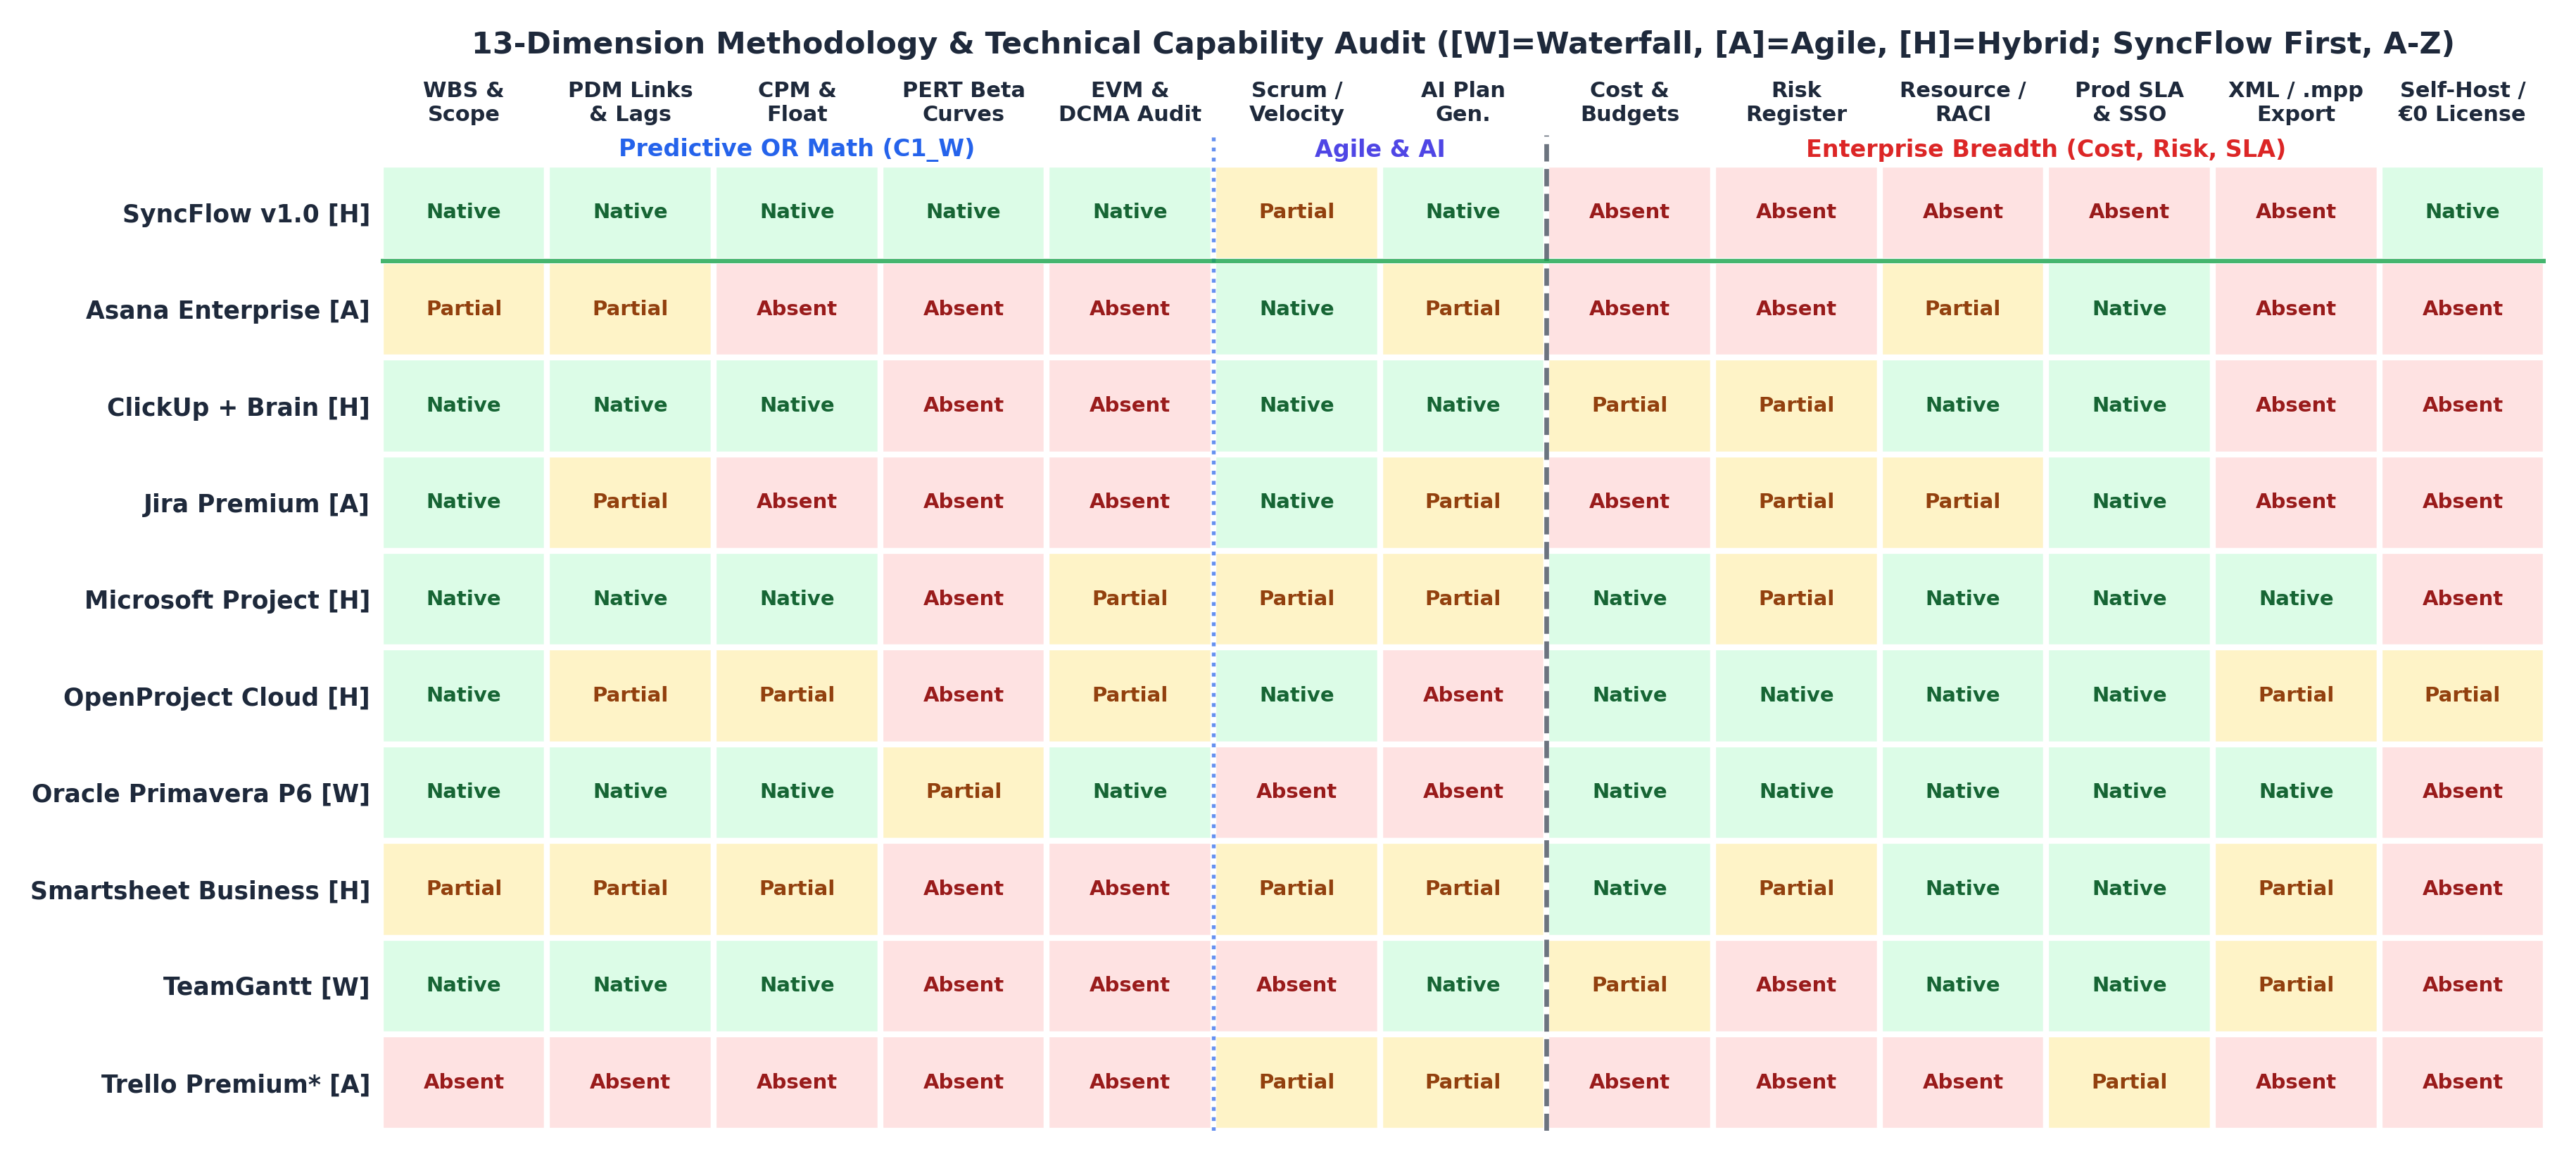
\includegraphics[width=1.0\textwidth]{images/va_capability_heatmap.png}
    \caption*{Thirteen-dimension audit classifying Waterfall [W], Agile [A], and Hybrid [H] platforms (SyncFlow first, commercial A--Z).}
\end{figure}

Three structural patterns separate the contenders:
\begin{enumerate}[leftmargin=2.3em,labelsep=0.6em]
    \item \textbf{Hybrid Core With Planned \textit{v2.0} Modules}: \textit{SyncFlow v1.0} pairs predictive PMBOK Chapter 6 scheduling (PDM lags, CPM, PERT, EVM, all 14 DCMA audits) with live WIP stopwatch execution. Financial budgets, Risk + Monte Carlo tools, SCRUM sprint boards, and XML/PDF exports remain deferred to the planned \textit{v2.0} upgrades;

    \vspace{1mm}

    \item \textbf{Clear Archetype Specialization}: Pure Agile tools such as \textit{Jira Premium} lead sprint velocity and CI/CD traceability without native CPM float math. Conversely, \textit{Oracle Primavera P6} and \textit{TeamGantt + AI} prioritize deterministic timelines, while Hybrid leaders such as \textit{OpenProject Cloud} natively balance Gantt planning and SCRUM boards;

    \vspace{1mm}

    \item \textbf{Operational Maturity Deficit in \textit{v1.0}}: Today, \textit{SyncFlow v1.0} lacks monetary Cost budgets, Risk Registers, RACI views, vendor SLAs, HTTPS TLS defaults, SMTP password recovery, vendored JS bundles, and automated CI tests.
\end{enumerate}

\subsubsection{Analytical Operations Research Rigor ($C_{1,W} = 4.5$)}
\textit{SyncFlow v1.0} earns an anchored rating of $C_{1,W} = 4.5$ by delivering two mathematical scheduling capabilities that are virtually absent from mainstream commercial tools without expensive external plugins:
\begin{itemize}[itemsep=1pt,topsep=1pt]
    \item \textbf{Interactive PERT Engine}: Continuous completion probabilities along the Critical Path ($CP$) are computed using the closed-form Gaussian error function integral:
    \begin{equation*}
        P(T \le t) = \frac{1}{2}\left[1 + \text{erf}\left(\frac{t - \mu_{CP}}{\sigma_{CP}\sqrt{2}}\right)\right], \quad \mu_{CP} = \sum_{j \in CP} \mu_j, \quad \sigma_{CP}^2 = \sum_{j \in CP} \sigma_j^2
    \end{equation*}
    Interactive P50, P80, and P90 sliders allow project managers to determine deadline confidence dynamically. Mainstream commercial suites (MS Project, ClickUp, Jira, Asana, Smartsheet) require external simulation add-ons (such as Full Monte or Risky\-Project) to calculate stochastic completion distributions;
    \item \textbf{Earned Value "Banana Envelope" S-Curve}: The scheduling engine natively graphs cumulative Planned Value bounds between early dates ($PV_{\text{Early}}$, Early Starts) and late dates ($PV_{\text{Late}}$, Late Starts), defining the mathematical confidence envelope for schedule slippage under PMBOK Process 6.5;
    \item \textbf{Automated DCMA 14-Point Schedule Audit}: The audit engine actively evaluates the schedule against all 14 DCMA metrics in \textit{v1.0} (including Metric~5 Hard Constraints, auditing rigid date constraints against project-level external deadlines in schedule settings), while interactive user-interface date locks for individual milestone overrides expand in planned \textit{v2.0}.
\end{itemize}

\subsubsection{Execution Quality Control \& Four-Stage Controller Verification (Process 6.6)}
Mainstream work management tools (e.g., Trello, Asana, Smartsheet) allow any user to arbitrarily mark tasks as "Done" or input subjective percentage completions that distort Earned Value tracking. To guarantee reporting integrity, \textit{SyncFlow} enforces a mandatory \textbf{Four-Stage Quality Control Workflow}:
\begin{equation*}
    \text{Not Started} \;\xrightarrow{\quad}\; \text{WIP} \;\xrightarrow{\quad}\; \text{Completed Pending Review} \;\xrightarrow{\quad}\; \text{Verified}
\end{equation*}
When a Team Member completes an activity, they must attach auditable deliverable evidence. Progress does not credit Earned Value ($EV$) until one of the \textbf{2 designated Project Controllers} (formally budgeted in our 25-user baseline) reviews the deliverable and approves verification or returns the task to "WIP" with corrective feedback.

\subsubsection{Multi-Modal Duration Estimation \& Portfolio Management}
Duration estimation supports \textbf{four operational modes}: Single-Point, Three-Point PERT ($t_e = \frac{o + 4m + p}{6}$), Parametric ($Q \times R$), and \textbf{Analogous Estimation} (which dynamically queries historical verified actuals from \texttt{/completed-activities}). Multi-project governance is coordinated through a \textbf{Reusable Teams Library} (\texttt{/syncflow/teams}) and an executive \textbf{Portfolio Dashboard} (\texttt{/syncflow/portfolio/dashboard}) summarizing cross-project critical path health and variance indicators.

\subsubsection{Bifurcated Persona UX \& Cognitive Adoption Friction ($C_3$)}
In project management software, organizations routinely suffer from a usability dichotomy between two extremes. On one end, lightweight task trackers (\textit{Asana}, \textit{ClickUp}, \textit{Smartsheet}) offer high usability ($C_3 = 4.0\text{--}4.5$) but lack deterministic Operations Research algorithms. On the opposite end, heavy enterprise suites such as \textit{Oracle Primavera P6} ($C_3 = 3.0$) and \textit{Microsoft Project Plan 3} ($C_3 = 3.5$) support formal CPM networks, but suffer from extreme learning curves, dense dialog trees, and monolithic tabular layouts. When frontline contributors are forced into these tools, cognitive fatigue and interface complexity discourage daily adoption, resulting in stale schedules, arbitrary progress guesses, or heavy organizational resistance.

\textit{SyncFlow} resolves this structural tension by enforcing a \textbf{Bifurcated Persona Architecture} that completely separates executive governance from operational execution:
\begin{itemize}[itemsep=1pt,topsep=1pt]
    \item \textbf{Project Managers \& Controllers (Governance Persona)}: Access the comprehensive 6-process PMBOK pipeline: interactive topological graphs, CPM early/late float bars, continuous Gaussian PERT probability sliders, EVM Banana Envelopes, DCMA audit scorecards, and formal deliverable verification gates;
    \item \textbf{Team Members (Frontline Execution Persona)}: Receive a streamlined, distraction-free operational task agenda with zero scheduling math clutter. Each assigned activity features a one-click live stopwatch timer, deliverable proof attachment, and status toggle.
\end{itemize}
By confining mathematical complexity to the 3 Project Managers and 2 Controllers, \textit{SyncFlow} allows the 20 operational Team Members to begin logging verified progress on day one without formal training, earning an anchored rating of $C_3 = 4.0$ (advancing to $4.5$ in planned \textit{v2.0} with sprint boards and mobile responsiveness).

\vspace{3mm}

\section{Financial Cost Breakdown}
Internal Make ownership eliminates software royalties, making internal engineering labor rather than cloud hosting \textit{SyncFlow}'s primary three-year expense. Applying Section 2.6's five-component identity across $N = 25$ seats, $t = 36$ months, foreign-exchange rate $r_{\text{fx}} = 0.92\text{ EUR/USD}$, and EU ICT labor rate $w_h = \text{€45/h}$ \cite{eurostat} yields exact closed-form cost equations for every contender:
$$
    \text{TCO}_{3\text{yr},i} = C_{\text{license},i} + C_{\text{infra/API},i} + C_{\text{deploy},i} + C_{\text{future},i} + C_{\text{maint},i}
$$

\begin{itemize}[itemsep=1pt,topsep=1pt]
    \item \textbf{Commercial License Formulas ($C_{\text{license},i}$)}: Seat-based USD plans scale linearly as $C_{\text{license},i} = N \cdot t \cdot p_{\text{mo},i} \cdot r_{\text{fx}}$ (omitting $r_{\text{fx}}$ for EUR tiers such as \textit{OpenProject}), whereas project-tier \textit{TeamGantt} bundles unlimited seats under $P = 15$ active projects via $(p_{\text{base}} + (P - 5) \cdot \Delta p_{\text{proj}}) \cdot t \cdot r_{\text{fx}} = (\$95 + 10 \times \$19) \times 36 \times 0.92 = \text{€9,439.20} \approx \text{€9,440}$;
    
    \vspace{1mm}
    
    \item \textbf{Internal Self-Hosted Baseline ($C_{\text{infra/API}}, C_{\text{deploy}}, C_{\text{future}}, C_{\text{maint}}$)}: Under standard managerial accounting, the 53-calendar-day project window (with software completed on November 9 after 36 active development days / 252 engineering hours, valuing initial R\&D at €11,340) is treated as an unrecoverable sunk cost ($C_{\text{license}} = 0, C_{\text{future}} = 0$). Its 36-month operational cost consists solely of cash hosting $C_{\text{infra/API}} = (28 + 6 + 8) \times 36 + 120 = \text{€1,632}$ (VPS, daily off-site encrypted backups, DNS/SMTP, and paid Gemini reserve), basic pre-rollout security hardening $C_{\text{deploy}} = 36\text{h} \times 45 = \text{€1,620}$, and regular maintenance/patching $C_{\text{maint}} = (2 \times 36)\text{h} \times 45 = \text{€3,240}$, establishing an audited unextended baseline of $\text{TCO}_{\text{v1.0}} = \textbf{€6,492}$. (If an organization were to build \textit{SyncFlow} from scratch today as a greenfield project, funding those 252 hours at €45/h would add €11,340, yielding a total greenfield build-and-run cost of $\approx \textbf{€17,832}$, matching mid-tier commercial suites like \textit{Jira Premium} at €17,084. For \textit{SyncFlow v2.0 Internal Make}, the 400 hours of planned development represent new uncommitted labor ($C_{\text{future}} = 400\text{h} \times 45 = \text{€18,000}$) to implement monetary EVM, Monte Carlo risk simulation, Scrum boards, and MS Project XML parsing, yielding $\text{TCO}_{\text{v2.0}} = \textbf{€24,492}$, evaluated in Section 3.6);
    
    \vspace{1mm}
    
    \item \textbf{External Reference Benchmark ($\text{TCO}_{\text{ref}}$)}: \textit{OpenProject Cloud Basic} minimizes qualifying commercial vendor TCO at $\text{TCO}_{\text{ref}} = \text{€8,655}$, setting the external denominator for Section 2.6's $s_{i,6}$ financial efficiency index. (While OpenProject offers a free self-hosted Community Edition, the paid plan is required to unlock paywalled enterprise baselines and Agile Scrum boards, as established in Section 3.1). For \textit{Jira Premium}, strict CPM compliance requires a €2,800 Marketplace CPM plugin ($\text{TCO}_{\text{cpm}} = 17,084 + 2,800 = \text{€19,884}$). Commercialized \textit{SyncFlow v2.0 SaaS} ($25 \times \text{€10} \times 36 + 1,620 + 1,080 = \text{€11,700}$) models buyer-side procurement, while the underlying provider-side development amortization and five-tier SaaS operating structure are analyzed in Section 3.6;

    \vspace{1mm}

    \item \textbf{Hidden Organizational Adoption and Training Friction}: While $C_{\text{deploy}}$ standardizes baseline administrative onboarding at 36 hours (€1,620), candidate platforms exhibit drastically divergent human learning curves. Monolithic suites like \textit{Oracle Primavera P6} ($C_3=3.0$) and \textit{Microsoft Project} ($C_3=3.5$) impose severe training barriers on frontline contributors, routinely demanding vendor-certified training programs (€1,500--€2,500/seat) or driving staff disengagement. Conversely, \textit{SyncFlow}'s bifurcated role design restricts cognitive complexity to the 3 Project Managers and 2 Controllers, allowing the 20 operational Team Members to track time on day one without formal training, protecting the organization against hidden adoption cost blowouts.
\end{itemize}

\begin{table}[H]
\centering
\scriptsize
\setlength{\tabcolsep}{2.2pt}
\renewcommand{\arraystretch}{1.18}
\caption*{Mathematical Derivation and 3-Year Economic TCO Breakdown Across Baseline Finalists (EUR, $N=25, t=36$).}
\begin{tabularx}{\textwidth}{>{\raggedright\arraybackslash}p{3.0cm} >{\raggedright\arraybackslash}p{3.4cm} r r r r r r c}
\toprule
\textbf{Vendor Platform} & \textbf{License / Labor Formula} & \textbf{Lic.} & \textbf{Infra} & \textbf{Deploy} & \textbf{Fut.} & \textbf{Maint.} & \textbf{TCO} & \textbf{Src} \\
\midrule
\textbf{\textit{SyncFlow v1.0 (Baseline)}} & $0 + 42(36){+}120 + 108\text{h}{\cdot}\text{€45}$ & \textbf{€0} & \textbf{€1,632} & \textbf{€1,620} & \textbf{€0} & \textbf{€3,240} & \textbf{€6,492} & \cite{eurostat} \\
\textit{Asana Ent. (est.)} & $25 \cdot \$35 \cdot 36 \cdot 0.92$ & €28,980 & €0 & €2,200 & €0 & €1,800 & \textbf{€32,980} & \cite{asana} \\
\textit{ClickUp + Brain} & $25 \cdot (\$12{+}\$9) \cdot 36 \cdot 0.92$ & €17,388 & €0 & €2,500 & €0 & €1,500 & \textbf{€21,388} & \cite{clickup} \\
\textit{Jira Premium}* & $25 \cdot \$15.56 \cdot 36 \cdot 0.92$ & €12,884 & €0 & €2,400 & €0 & €1,800 & \textbf{€17,084} & \cite{jira} \\
\textit{MS Project Plan 3} & $25 \cdot \$30 \cdot 36 \cdot 0.92$ & €24,840 & €0 & €2,000 & €0 & €2,000 & \textbf{€28,840} & \cite{msproject} \\
\textit{OpenProject Basic} & $25 \cdot \text{€5.95} \cdot 36$ & €5,355 & €0 & €1,800 & €0 & €1,500 & \textbf{€8,655} & \cite{openproject} \\
\textit{Primavera P6 Cloud} & $25 \cdot \$125 \cdot 36 \cdot 0.92$ & €103,500 & €0 & €22,000 & €0 & €12,000 & \textbf{€137,500} & \cite{primavera} \\
\textit{Smartsheet Business} & $25 \cdot \$19 \cdot 36 \cdot 0.92$ & €15,732 & €0 & €1,800 & €0 & €1,400 & \textbf{€18,932} & \cite{smartsheet} \\
\textit{TeamGantt + AI} & $(\$95 {+} 10{\cdot}\$19) \cdot 36 \cdot 0.92$ & €9,440 & €0 & €1,200 & €0 & €900 & \textbf{€11,540} & \cite{teamgantt} \\
\bottomrule
\end{tabularx}
\end{table}

\begin{figure}[H]
    \centering
    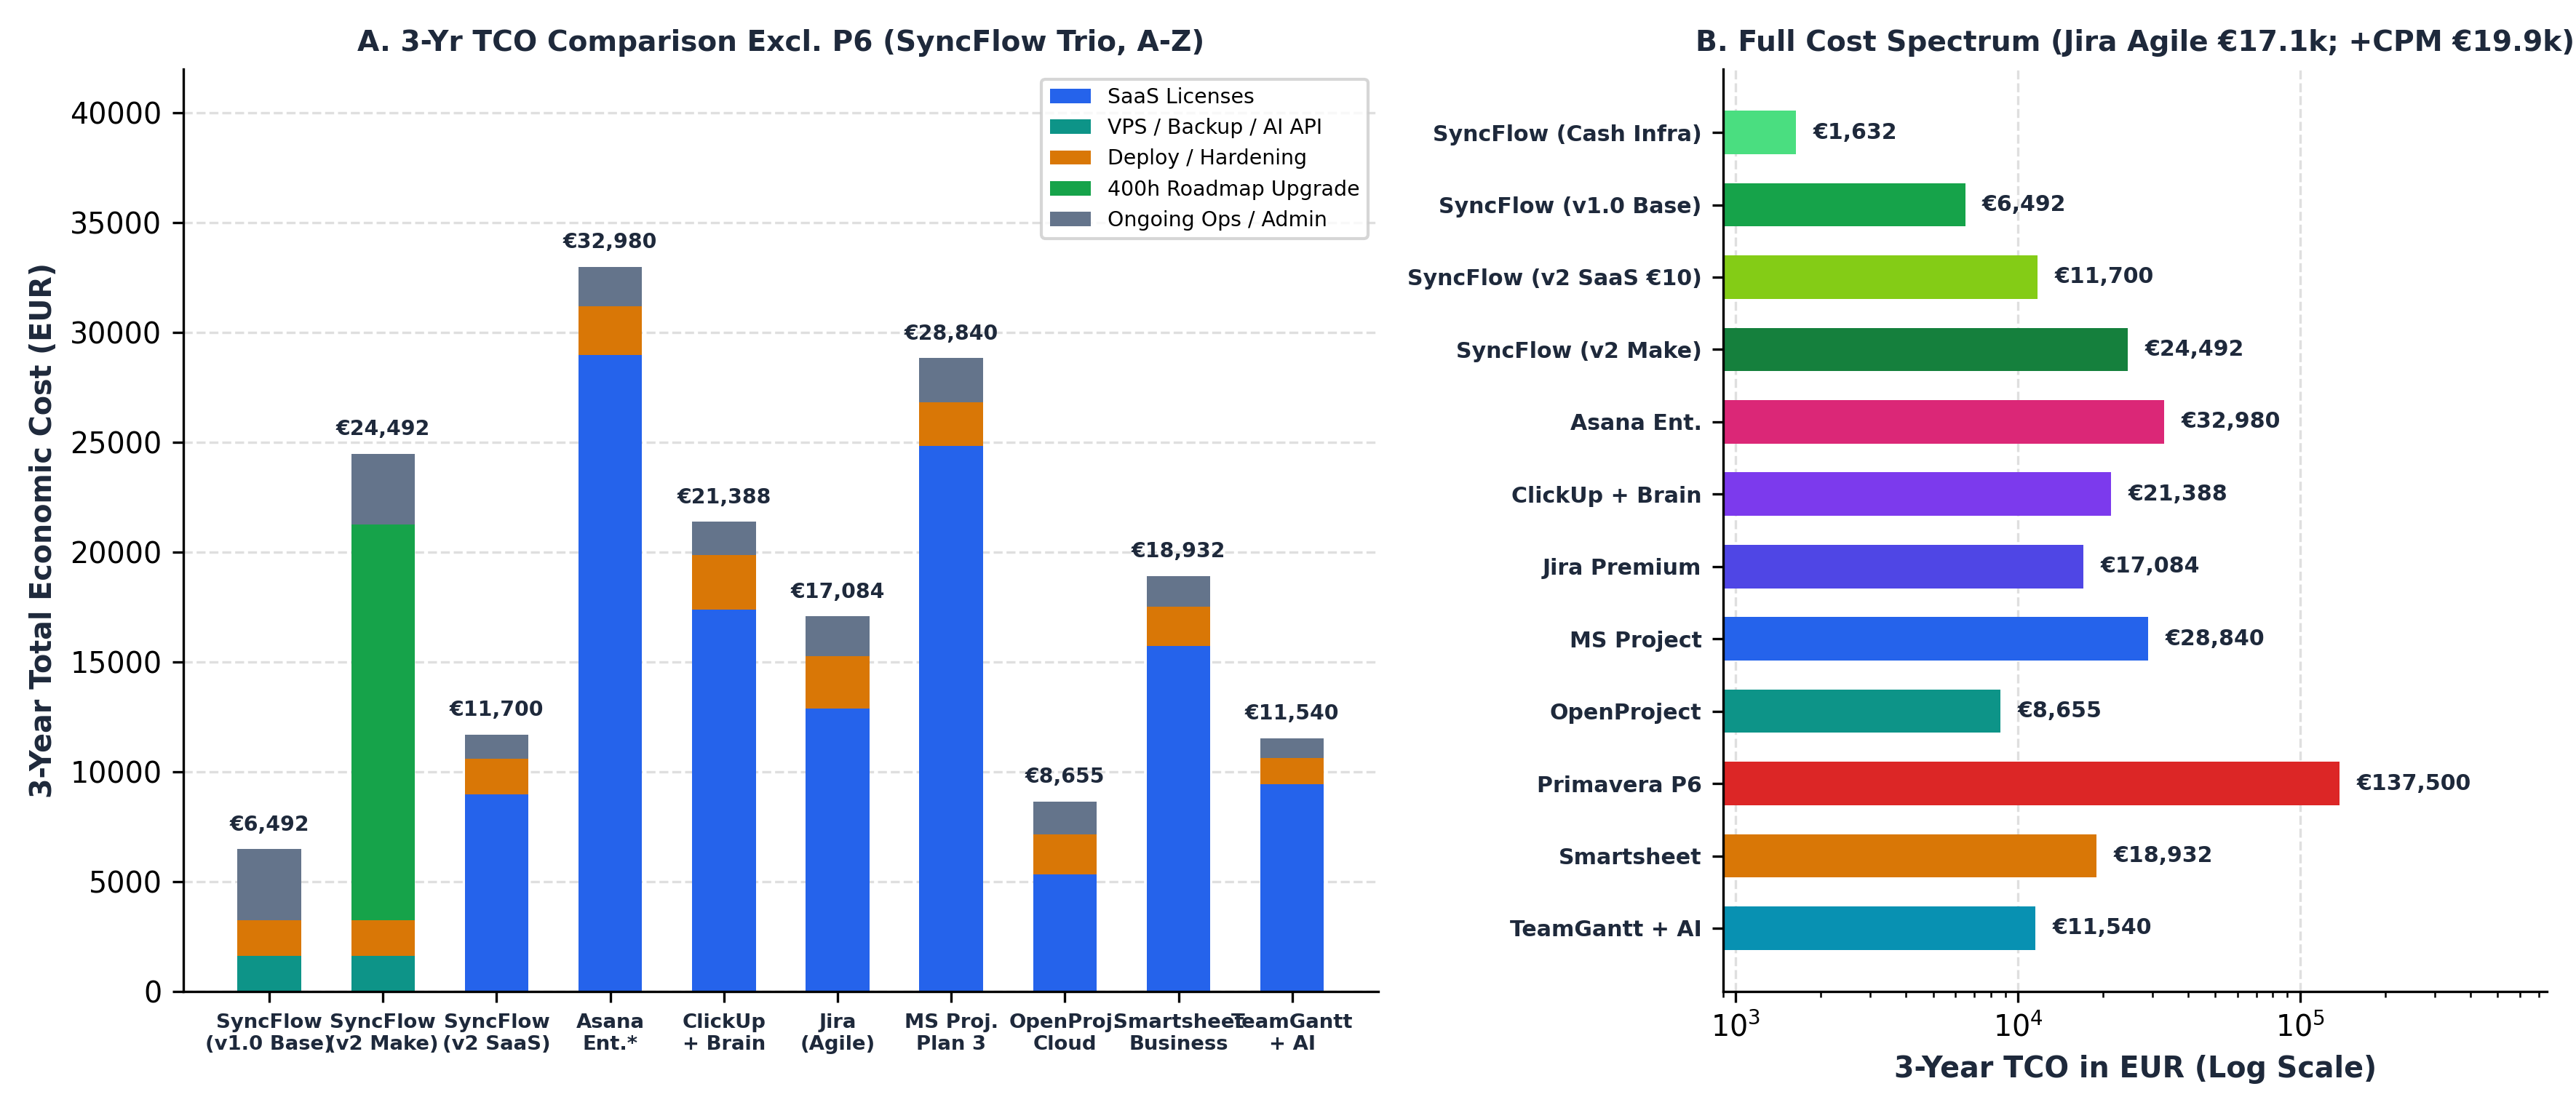
\includegraphics[width=1.0\textwidth]{images/va_tco_3yr.png}
    \caption*{Realistic three-year economic TCO breakdown ordered SyncFlow first then A--Z (Panel A) and cash-only vs. full-roadmap contrast (Panel B).}
\end{figure}

Three financial patterns shape cost efficiency before scoring begins:
\begin{itemize}[itemsep=1pt,topsep=1pt]
    \item \textbf{Cash Outlay vs. Full Economic Labor}: Direct cash hosting equals only €1,632 over three years, while basic deployment and maintenance bring \textit{SyncFlow v1.0}'s baseline TCO to €6,492. (The planned 400-hour v2.0 upgrade roadmap brings the full Make investment to €24,492, evaluated in Section 3.6);
    \item \textbf{Sixteenfold Commercial Cost Spread}: Three-Year Total Cost of Ownership ranges from €8,655 to €137,500 across the evaluated commercial platforms, driven by enterprise per-seat rates and mandatory onboarding fees;
    \item \textbf{Baseline Cost Rank}: Low licensing places \textit{OpenProject}, \textit{TeamGantt}, and \textit{SyncFlow} cleanly ahead of mainstream proprietary subscriptions before technical weights apply.
\end{itemize}

\newpage

\section{Metric Calculation Across Candidate Platforms}
Applying Chapter 2's five equations transparently transforms each candidate's half-point votes and Section 3.3 TCO into final evaluation indices prior to ranking. Below, each application is detailed individually to verify all intermediate and final scores ($C_1^*$, $s_6$, $\text{Tech}$, $Q_{\text{fair}}$, $\text{CPP}$, $S_{\text{fair}}$, and $S_{\text{CPM}}$).

\subsubsection{SyncFlow v1.0 (Baseline)}
\textbf{Parameters}: Hybrid ($\alpha = 0.60$), $(C_{1,W}, C_{1,A}) = (4.5, 3.5)$, $(C_2, C_3, C_4, C_5) = (2.5, 4.0, 2.0, 5.0)$, $\text{TCO} = \text{€6,492}$.
\begin{small}
\begin{align*}
    C_1^* &= 0.60(4.5) + 0.40(3.5) = \mathbf{4.10} \qquad \qquad
    s_6 = \text{round}_1\!\left(\min\left(5.0, 5.0 - 2.6\log_{10}\!\tfrac{6492}{8655}\right)\right) = \mathbf{5.0} \\
    \text{Tech} &= 0.25(4.10) + 0.15(2.5 + 4.0 + 2.0) + 0.10(5.0) = 2.800 \qquad \qquad
    Q_{\text{fair}} = \tfrac{2.800}{0.80} = \mathbf{3.50} \\
    \text{CPP} &= \tfrac{6492}{3.50} = \mathbf{\text{€1,855/pt}} \qquad \qquad
    S_{\text{fair}} = 2.800 + 0.20(5.0) = \mathbf{3.80} \\
    S_{\text{CPM}} &= 0.25(4.5) + 0.15(2.5 + 4.0 + 2.0) + 0.10(5.0) + 0.20(5.0) = 2.900 + 1.000 = \mathbf{3.90}
\end{align*}
\end{small}

\subsubsection{OpenProject (Cloud Basic)}
\textbf{Parameters}: Hybrid ($\alpha = 0.60$), $(C_{1,W}, C_{1,A}) = (3.5, 4.0)$, $(C_2, C_3, C_4, C_5) = (4.5, 3.5, 4.5, 4.0)$, $\text{TCO} = \text{€8,655}$.
\begin{small}
\begin{align*}
    C_1^* &= 0.60(3.5) + 0.40(4.0) = \mathbf{3.70} \qquad \qquad
    s_6 = \text{round}_1\!\left(5.0 - 2.6\log_{10}\!\tfrac{8655}{8655}\right) = \mathbf{5.0} \\
    \text{Tech} &= 0.25(3.70) + 0.15(4.5 + 3.5 + 4.5) + 0.10(4.0) = 3.200 \qquad \qquad
    Q_{\text{fair}} = \tfrac{3.200}{0.80} = \mathbf{4.00} \\
    \text{CPP} &= \tfrac{8655}{4.00} = \mathbf{\text{€2,164/pt}} \qquad \qquad
    S_{\text{fair}} = 3.200 + 0.20(5.0) = \mathbf{4.20} \\
    S_{\text{CPM}} &= 0.25(3.5) + 0.15(4.5 + 3.5 + 4.5) + 0.10(4.0) + 0.20(5.0) = \mathbf{4.15}
\end{align*}
\end{small}

\subsubsection{Jira Premium (Atlassian)}
\textbf{Parameters}: Agile ($\alpha = 0.30$), $(C_{1,W}, C_{1,A}) = (2.5, 5.0)$, $(C_2, C_3, C_4, C_5) = (4.0, 4.0, 4.5, 2.5)$, native $\text{TCO} = \text{€17,084}$, strict CPM $\text{TCO}_{\text{cpm}} = \text{€19,884}$.
\begin{small}
\begin{align*}
    C_1^* &= 0.30(2.5) + 0.70(5.0) = \mathbf{4.25} \qquad \qquad
    s_6 = \text{round}_1\!\left(5.0 - 2.6\log_{10}\!\tfrac{17084}{8655}\right) = \mathbf{4.2} \\
    \text{Tech} &= 0.25(4.25) + 0.15(4.0 + 4.0 + 4.5) + 0.10(2.5) = 3.1875 \qquad \qquad
    Q_{\text{fair}} = \tfrac{3.1875}{0.80} = \mathbf{3.98} \\
    \text{CPP} &= \tfrac{17084}{3.98} = \mathbf{\text{€4,292/pt}} \qquad \qquad
    S_{\text{fair}} = 3.1875 + 0.20(4.2) = \mathbf{4.03} \\
    s_{6,\text{cpm}} &= \text{round}_1\!\left(5.0 - 2.6\log_{10}\!\tfrac{19884}{8655}\right) = \mathbf{4.1} \\
    S_{\text{CPM}} &= 0.25(2.5) + 0.15(4.0 + 4.0 + 4.5) + 0.10(2.5) + 0.20(4.1) = \mathbf{3.57}
\end{align*}
\end{small}

\subsubsection{ClickUp (Business + Brain)}
\textbf{Parameters}: Hybrid ($\alpha = 0.60$), $(C_{1,W}, C_{1,A}) = (3.5, 4.5)$, $(C_2, C_3, C_4, C_5) = (4.0, 4.5, 4.0, 2.0)$, $\text{TCO} = \text{€21,388}$.
\begin{small}
\begin{align*}
    C_1^* &= 0.60(3.5) + 0.40(4.5) = \mathbf{3.90} \qquad \qquad
    s_6 = \text{round}_1\!\left(5.0 - 2.6\log_{10}\!\tfrac{21388}{8655}\right) = \mathbf{4.0} \\
    \text{Tech} &= 0.25(3.90) + 0.15(4.0 + 4.5 + 4.0) + 0.10(2.0) = 3.050 \qquad \qquad
    Q_{\text{fair}} = \tfrac{3.050}{0.80} = \mathbf{3.81} \\
    \text{CPP} &= \tfrac{21388}{3.81} = \mathbf{\text{€5,614/pt}} \qquad \qquad
    S_{\text{fair}} = 3.050 + 0.20(4.0) = \mathbf{3.85} \\
    S_{\text{CPM}} &= 0.25(3.5) + 0.15(4.0 + 4.5 + 4.0) + 0.10(2.0) + 0.20(4.0) = \mathbf{3.75}
\end{align*}
\end{small}

\subsubsection{TeamGantt (Business + AI)}
\textbf{Parameters}: Waterfall ($\alpha = 0.85$), $(C_{1,W}, C_{1,A}) = (3.5, 2.0)$,\\ $(C_2, C_3, C_4, C_5) = (3.5, 4.5, 4.0, 2.0)$, $\text{TCO} = \text{€11,540}$.
\begin{small}
\begin{align*}
    C_1^* &= 0.85(3.5) + 0.15(2.0) = \mathbf{3.28} \qquad \qquad
    s_6 = \text{round}_1\!\left(5.0 - 2.6\log_{10}\!\tfrac{11540}{8655}\right) = \mathbf{4.7} \\
    \text{Tech} &= 0.25(3.28) + 0.15(3.5 + 4.5 + 4.0) + 0.10(2.0) = 2.820 \qquad \qquad
    Q_{\text{fair}} = \tfrac{2.820}{0.80} = \mathbf{3.53} \\
    \text{CPP} &= \tfrac{11540}{3.53} = \mathbf{\text{€3,269/pt}} \qquad \qquad
    S_{\text{fair}} = 2.820 + 0.20(4.7) = \mathbf{3.76} \\
    S_{\text{CPM}} &= 0.25(3.5) + 0.15(3.5 + 4.5 + 4.0) + 0.10(2.0) + 0.20(4.7) = 3.815 \to \mathbf{3.82}
\end{align*}
\end{small}

\subsubsection{Microsoft Project Plan 3}
\textbf{Parameters}: Hybrid ($\alpha = 0.60$), $(C_{1,W}, C_{1,A}) = (4.5, 3.5)$, $(C_2, C_3, C_4, C_5) = (4.0, 3.5, 4.5, 2.0)$, $\text{TCO} = \text{€28,840}$.
\begin{small}
\begin{align*}
    C_1^* &= 0.60(4.5) + 0.40(3.5) = \mathbf{4.10} \qquad \qquad
    s_6 = \text{round}_1\!\left(5.0 - 2.6\log_{10}\!\tfrac{28840}{8655}\right) = \mathbf{3.6} \\
    \text{Tech} &= 0.25(4.10) + 0.15(4.0 + 3.5 + 4.5) + 0.10(2.0) = 3.025 \qquad \qquad
    Q_{\text{fair}} = \tfrac{3.025}{0.80} = \mathbf{3.78} \\
    \text{CPP} &= \tfrac{28840}{3.78} = \mathbf{\text{€7,630/pt}} \qquad \qquad
    S_{\text{fair}} = 3.025 + 0.20(3.6) = \mathbf{3.75} \\
    S_{\text{CPM}} &= 0.25(4.5) + 0.15(4.0 + 3.5 + 4.5) + 0.10(2.0) + 0.20(3.6) = \mathbf{3.85}
\end{align*}
\end{small}

\subsubsection{Smartsheet Business}
\textbf{Parameters}: Hybrid ($\alpha = 0.60$), $(C_{1,W}, C_{1,A}) = (3.0, 3.0)$, $(C_2, C_3, C_4, C_5) = (4.0, 4.0, 4.5, 2.0)$, $\text{TCO} = \text{€18,932}$.
\begin{small}
\begin{align*}
    C_1^* &= 0.60(3.0) + 0.40(3.0) = \mathbf{3.00} \qquad \qquad
    s_6 = \text{round}_1\!\left(5.0 - 2.6\log_{10}\!\tfrac{18932}{8655}\right) = \mathbf{4.1} \\
    \text{Tech} &= 0.25(3.00) + 0.15(4.0 + 4.0 + 4.5) + 0.10(2.0) = 2.825 \qquad \qquad
    Q_{\text{fair}} = \tfrac{2.825}{0.80} = \mathbf{3.53} \\
    \text{CPP} &= \tfrac{18932}{3.53} = \mathbf{\text{€5,363/pt}} \qquad \qquad
    S_{\text{fair}} = 2.825 + 0.20(4.1) = \mathbf{3.65} \\
    S_{\text{CPM}} &= 0.25(3.0) + 0.15(4.0 + 4.0 + 4.5) + 0.10(2.0) + 0.20(4.1) = \mathbf{3.65}
\end{align*}
\end{small}

\subsubsection{Oracle Primavera P6 Cloud}
\textbf{Parameters}: Waterfall ($\alpha = 0.85$), $(C_{1,W}, C_{1,A}) = (5.0, 1.0)$,\\ $(C_2, C_3, C_4, C_5) = (5.0, 3.0, 5.0, 1.5)$, $\text{TCO} = \text{€137,500}$.
\begin{small}
\begin{align*}
    C_1^* &= 0.85(5.0) + 0.15(1.0) = \mathbf{4.40} \qquad \qquad
    s_6 = \text{round}_1\!\left(5.0 - 2.6\log_{10}\!\tfrac{137500}{8655}\right) = \mathbf{1.9} \\
    \text{Tech} &= 0.25(4.40) + 0.15(5.0 + 3.0 + 5.0) + 0.10(1.5) = 3.200 \qquad \qquad
    Q_{\text{fair}} = \tfrac{3.200}{0.80} = \mathbf{4.00} \\
    \text{CPP} &= \tfrac{137500}{4.00} = \mathbf{\text{€34,375/pt}} \qquad \qquad
    S_{\text{fair}} = 3.200 + 0.20(1.9) = \mathbf{3.58} \\
    S_{\text{CPM}} &= 0.25(5.0) + 0.15(5.0 + 3.0 + 5.0) + 0.10(1.5) + 0.20(1.9) = \mathbf{3.73}
\end{align*}
\end{small}

\subsubsection{Asana Enterprise (est.)}
\textbf{Parameters}: Agile ($\alpha = 0.30$), $(C_{1,W}, C_{1,A}) = (2.0, 4.0)$, $(C_2, C_3, C_4, C_5) = (3.5, 4.0, 4.5, 2.0)$, $\text{TCO} = \text{€32,980}$.
\begin{small}
\begin{align*}
    C_1^* &= 0.30(2.0) + 0.70(4.0) = \mathbf{3.40} \qquad \qquad
    s_6 = \text{round}_1\!\left(5.0 - 2.6\log_{10}\!\tfrac{32980}{8655}\right) = \mathbf{3.5} \\
    \text{Tech} &= 0.25(3.40) + 0.15(3.5 + 4.0 + 4.5) + 0.10(2.0) = 2.850 \qquad \qquad
    Q_{\text{fair}} = \tfrac{2.850}{0.80} = \mathbf{3.56} \\
    \text{CPP} &= \tfrac{32980}{3.56} = \mathbf{\text{€9,264/pt}} \qquad \qquad
    S_{\text{fair}} = 2.850 + 0.20(3.5) = \mathbf{3.55} \\
    S_{\text{CPM}} &= 0.25(2.0) + 0.15(3.5 + 4.0 + 4.5) + 0.10(2.0) + 0.20(3.5) = \mathbf{3.20}
\end{align*}
\end{small}

\newpage

\section{Methodology-Aware Rankings Scorecards}
SyncFlow was rated manually to ensure rigorous critical scrutiny. This evaluation preceded the use of \texttt{Gemini-4-Argon} to assess the votes of the remaining applications, minimising potential bias. This approach was primarily driven by time constraints, which made independent evaluation of all applications or Large Language Model assessment of the entire project impractical.

\begin{table}[H]
\centering
\scriptsize
\setlength{\tabcolsep}{2.2pt}
\renewcommand{\arraystretch}{1.04}
\caption*{Forward-Looking Baseline Scorecard: Make -- Existing Asset vs. Buy (Sorted Descending by $S_{\text{fair}}$, Ranks 1--9).}
\begin{tabularx}{\textwidth}{>{\raggedright\arraybackslash}X l c c c c c c c c c c}
\toprule
\textbf{Platform} & \textbf{Scenario} & \textbf{$C_{1,W}$} & \textbf{$C_{1,A}$} & \textbf{$C_1^*$} & \textbf{$C_2$} & \textbf{$C_3$} & \textbf{$C_4$} & \textbf{$C_5$} & \textbf{$C_6$} & \textbf{$S_{\text{fair}}$ (Rk)} & \textbf{$S_{\text{CPM}}$ (Rk)} \\
\midrule
\textit{OpenProject (Cloud Basic)} & Buy -- Comm. & 3.5 & 4.0 & 3.70 & 4.5 & 3.5 & 4.5 & 4.0 & \textbf{5.0} & \textbf{4.20 (1)} & \textbf{4.15 (1)} \\
\textit{Jira Premium (Atlassian)} & Buy -- Comm. & 2.5 & \textbf{5.0} & 4.25 & 4.0 & 4.0 & 4.5 & 2.5 & 4.2 & \textbf{4.03 (2)} & 3.57 (8) \\
\textit{ClickUp (Business + Brain)} & Buy -- Comm. & 3.5 & 4.5 & 3.90 & 4.0 & \textbf{4.5} & 4.0 & 2.0 & 4.0 & \textbf{3.85 (3)} & 3.75 (5) \\
\textbf{\textit{SyncFlow v1.0 (Baseline)}} & \textbf{Make -- Exist.} & 4.5 & 3.5 & 4.10 & 2.5 & 4.0 & 2.0 & \textbf{5.0} & \textbf{5.0} & \textbf{3.80 (4)} & \textbf{3.90 (2)} \\
\textit{TeamGantt (Business + AI)} & Buy -- Comm. & 3.5 & 2.0 & 3.28 & 3.5 & \textbf{4.5} & 4.0 & 2.0 & 4.7 & \textbf{3.76 (5)} & 3.82 (4) \\
\textit{Microsoft Project Plan 3} & Buy -- Comm. & 4.5 & 3.5 & 4.10 & 4.0 & 3.5 & 4.5 & 2.0 & 3.6 & \textbf{3.75 (6)} & 3.85 (3) \\
\textit{Smartsheet Business} & Buy -- Comm. & 3.0 & 3.0 & 3.00 & 4.0 & 4.0 & 4.5 & 2.0 & 4.1 & \textbf{3.65 (7)} & 3.65 (7) \\
\textit{Oracle Primavera P6 Cloud} & Buy -- Comm. & \textbf{5.0} & 1.0 & \textbf{4.40} & \textbf{5.0} & 3.0 & \textbf{5.0} & 1.5 & 1.9 & \textbf{3.58 (8)} & 3.73 (6) \\
\textit{Asana Enterprise (est.)} & Buy -- Comm. & 2.0 & 4.0 & 3.40 & 3.5 & 4.0 & 4.5 & 2.0 & 3.5 & \textbf{3.55 (9)} & 3.20 (9) \\
\bottomrule
\end{tabularx}

\vspace{1.5mm}

\setlength{\tabcolsep}{3.0pt}
\caption*{Greenfield Counterfactual Scorecard: Make -- Greenfield vs. Buy (All Evaluated From Scratch, Sorted by $S_{\text{fair}}$).}
\begin{tabularx}{\textwidth}{>{\raggedright\arraybackslash}X l c c c c c c}
\toprule
\textbf{Platform} & \textbf{Procurement Scenario} & \textbf{3-Yr TCO} & \textbf{$C_6$} & \textbf{$Q_{\text{fair}}$} & \textbf{CPP (€/pt)} & \textbf{$S_{\text{fair}}$ (Rk)} & \textbf{$S_{\text{CPM}}$ (Rk)} \\
\midrule
\textit{OpenProject (Cloud Basic)} & Buy -- Commercial Solution & €8,655 & \textbf{5.0} & 4.00 & €2,164 & \textbf{4.20 (1)} & \textbf{4.15 (1)} \\
\textit{Jira Premium (Atlassian)} & Buy -- Commercial Solution & €17,084 & 4.2 & 3.99 & €4,282 & \textbf{4.03 (2)} & 3.57 (8) \\
\textit{ClickUp (Business + Brain)} & Buy -- Commercial Solution & €21,388 & 4.0 & 3.81 & €5,614 & \textbf{3.85 (3)} & 3.75 (4) \\
\textit{TeamGantt (Business + AI)} & Buy -- Commercial Solution & €11,540 & 4.7 & 3.53 & €3,269 & \textbf{3.76 (4)} & 3.82 (3) \\
\textit{Microsoft Project Plan 3} & Buy -- Commercial Solution & €28,840 & 3.6 & 3.79 & €7,610 & \textbf{3.75 (5)} & 3.85 (2) \\
\textit{Smartsheet Business} & Buy -- Commercial Solution & €18,932 & 4.1 & 3.54 & €5,348 & \textbf{3.65 (6)} & 3.65 (7) \\
\textbf{\textit{SyncFlow v1.0 (Greenfield)}} & \textbf{Make -- Greenfield} & \textbf{€17,832} & 4.2 & 3.50 & €5,095 & \textbf{3.64 (7)} & \textbf{3.74 (5)} \\
\textit{Oracle Primavera P6 Cloud} & Buy -- Commercial Solution & €137,500 & 1.9 & \textbf{4.00} & €34,375 & \textbf{3.58 (8)} & 3.73 (6) \\
\textit{Asana Enterprise (est.)} & Buy -- Commercial Solution & €32,980 & 3.5 & 3.56 & €9,264 & \textbf{3.55 (9)} & 3.20 (9) \\
\bottomrule
\end{tabularx}
\end{table}

The empirical findings from both forward-looking and counterfactual evaluations illustrate how initial development investment influences comparative software economics. The dual scoring distributions and value efficiency dynamics are visualized and analyzed below.

\newpage

\begin{figure}[H]
    \centering
    \begin{minipage}[b]{0.65\textwidth}
        \centering
        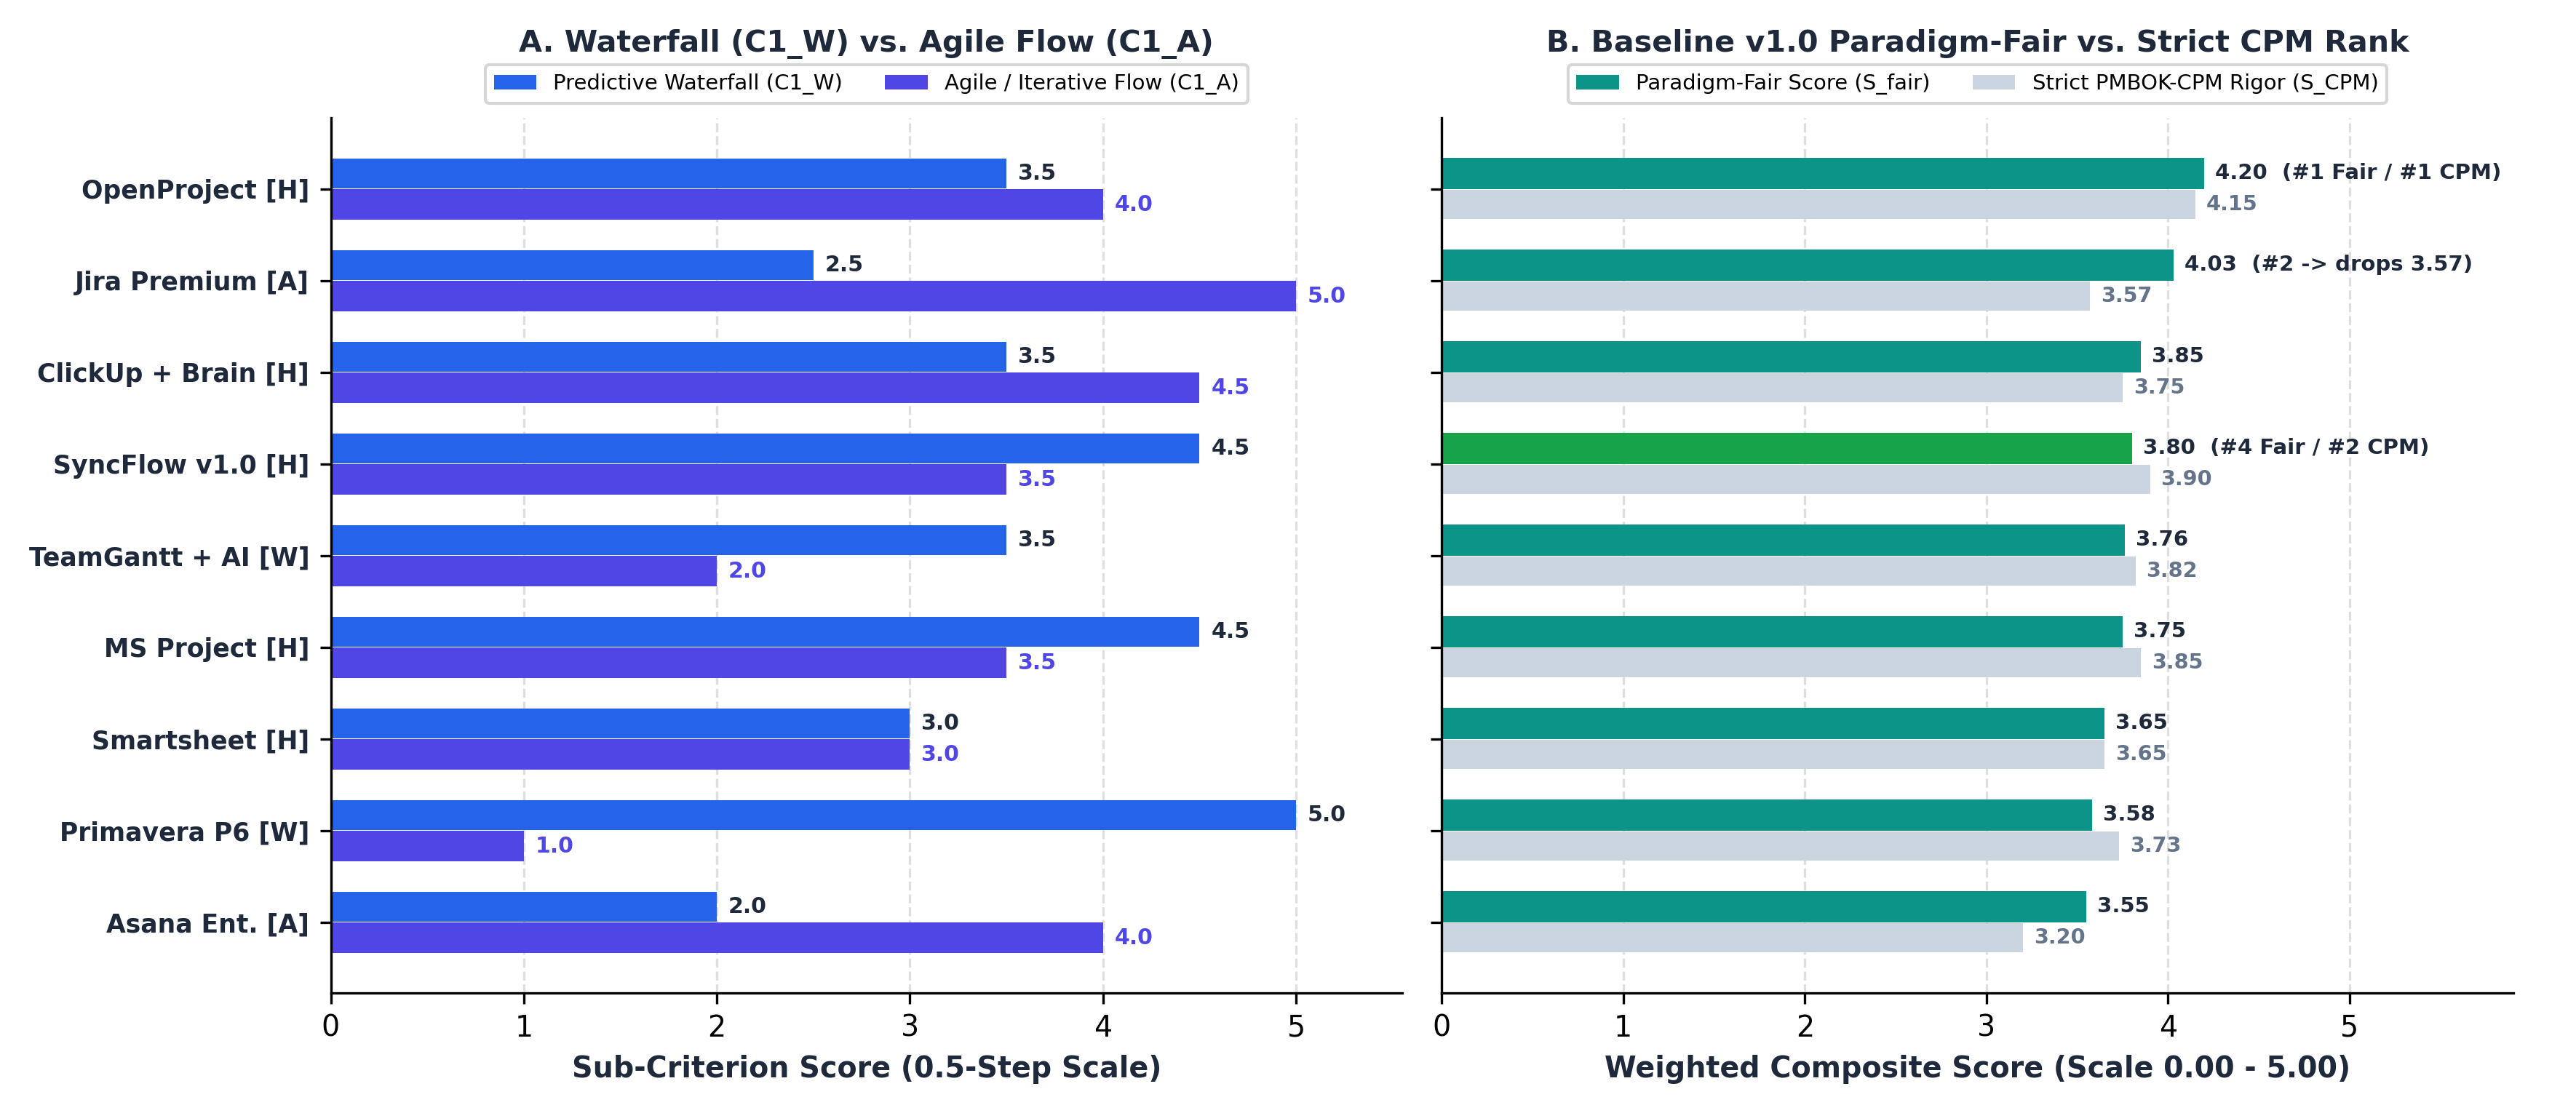
\includegraphics[width=\textwidth]{images/va_weighted_scores.png}
        \caption*{(a) Sub-scores \& Baseline Rankings.}
    \end{minipage}\hfill
    \begin{minipage}[b]{0.65\textwidth}
        \centering
        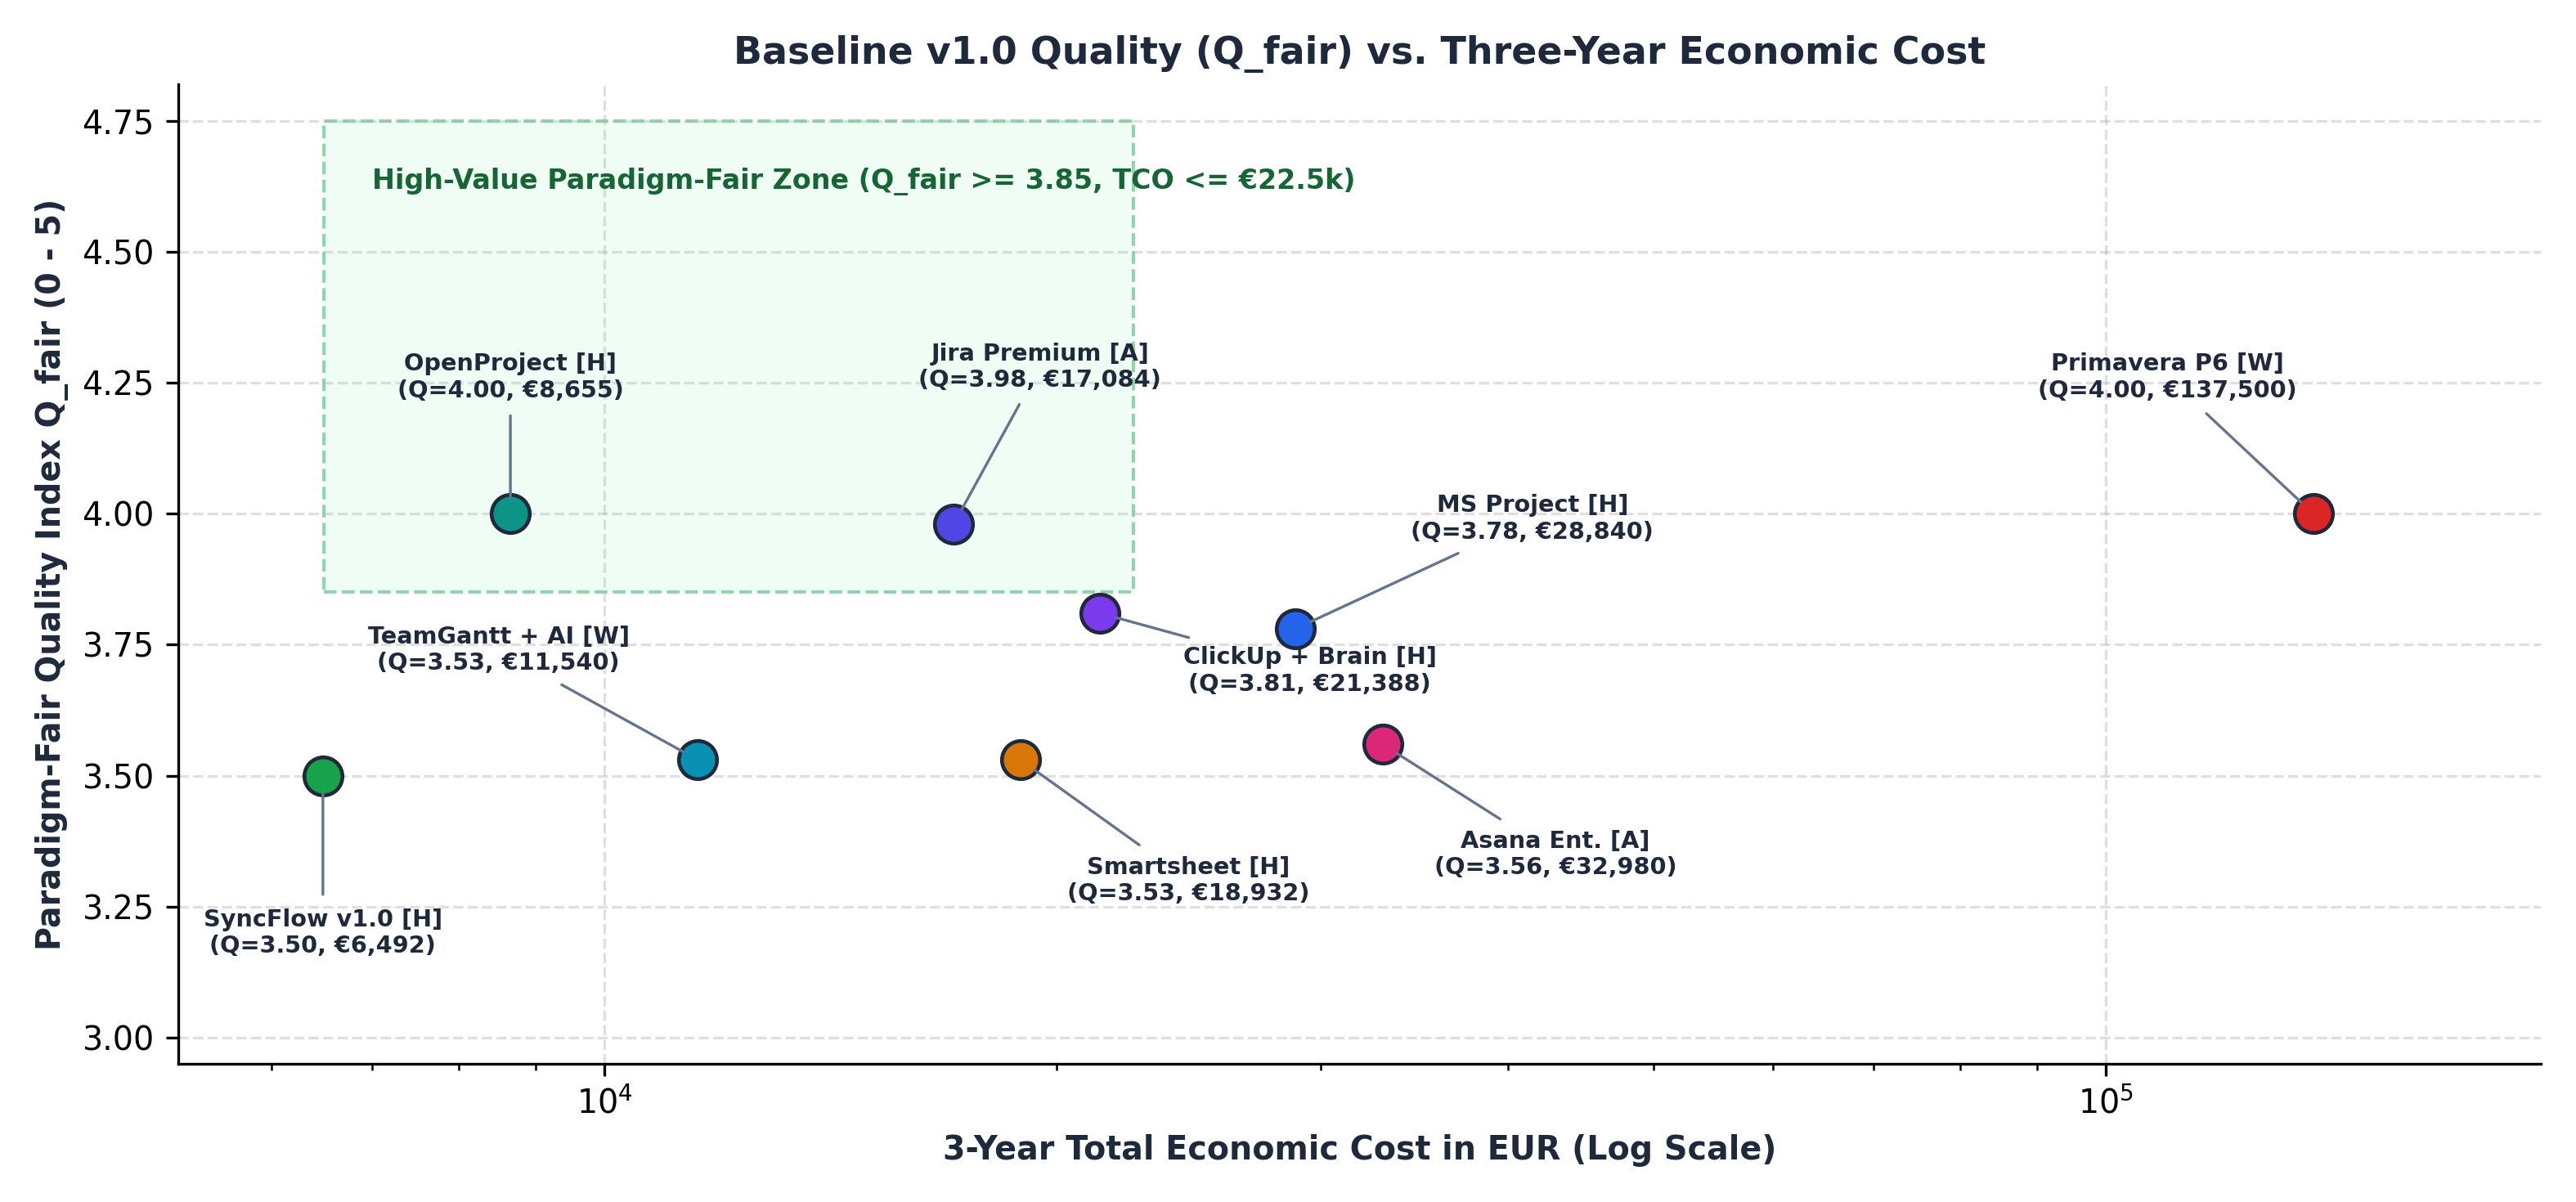
\includegraphics[width=\textwidth]{images/va_value_quadrant.png}
        \caption*{(b) Quality Index ($Q_{\text{fair}}$) vs. Three-Year TCO.}
    \end{minipage}
    \vspace{-1mm}
    \caption*{Dual-Lens Baseline Scoring Profiles and Value Efficiency Quadrant across all nine finalists.}
\end{figure}

Three core drivers explain these multi-scenario comparative rankings:
\begin{itemize}[itemsep=1.5pt,topsep=2pt]
    \item \textbf{Existing Asset vs. Greenfield Make Dynamics}: Under forward-looking \textit{Make -- Existing Asset} (Table 3.4), historical R\&D (€11,340) is sunk, leaving a lean €6,492 OpEx ($C_6 = 5.0$) that propels \textit{SyncFlow v1.0} to \textbf{Rank \#4 Fair (3.80)} and \textbf{Rank \#2 CPM (3.90)}. Conversely, under ex-ante \textit{Make -- Greenfield} (Table 3.5), absorbing full €11,340 development CapEx raises TCO to €17,832 ($C_6 = 4.2$), moving SyncFlow to \textbf{Rank \#7 Fair (3.64)} (closely behind Smartsheet at 3.65) and \textbf{Rank \#5 CPM (3.74)} (surpassing Primavera, Smartsheet, Jira, and Asana);
    \item \textbf{Commercial Champions Across Paradigms}: \textit{OpenProject Cloud} dominates both evaluations (\#1 Fair at 4.20, \#1 CPM at 4.15) via unencumbered pricing ($C_6 = 5.0$), open-core extensibility ($4.0$), and balanced governance. In contrast, \textit{Jira Premium} captures \#2 in Paradigm-Fair (4.03) on Agile velocity, but plunges to \#8 under Strict CPM (3.57);
    \item \textbf{Strict CPM Resilience}: SyncFlow embeds Kahn's topological sort and CPM forward and backward passes in native Python and NumPy. Its mathematical core remains robust even under Greenfield costing (\#5 CPM, 3.74), outscoring commercial suites lacking dependency rigor.
\end{itemize}

While the Greenfield counterfactual confirms that developing SyncFlow from scratch incurs substantial initial engineering expenditure, possessing the functional v1.0 prototype allows the enterprise to bypass this hurdle. However, to match premier commercial solutions in operational breadth, enterprise hardening, and automated governance, SyncFlow requires targeted evolutionary upgrades. This motivates the subsequent comparative analysis of the SyncFlow v2.0 development program.

\newpage

\section{SyncFlow 2.0 Comparative Analysis}
The planned \textit{SyncFlow v2.0} roadmap addresses functional and operational gaps identified in the baseline audit through a 400-hour development program (€18,000 at €45/h) over six months. The upgrade introduces PMBOK monetary Cost Management and EVM, a graph-wide Monte Carlo Risk Register, Agile SCRUM boards with burndown tracking, bidirectional MS Project XML/PDF export, and Gemini multimodal processing. Factoring in pre-rollout hardening (€1,620), hosting (€1,632), and three-year maintenance (€3,240), the resulting three-year Total Cost of Ownership is \textbf{€24,492} ($C_6 = 3.8$). 

\vspace{3mm}

Two deployment configurations are evaluated:
\begin{itemize}[itemsep=1pt,topsep=1.5pt]
	\item \textbf{\textit{SyncFlow v2.0 (Internal Make)}}: The enterprise develops, self-hosts, and maintains the platform internally, preserving complete source-code custody and open-source sovereignty ($C_5 = 5.0, C_6 = 3.8$, $\text{TCO} = \text{€24,492}$);
	\item \textbf{\textit{SyncFlow v2.0 (Commercial SaaS, €10/user/month)}}: Evaluates the system as a turnkey commercial subscription. For 25 seats over 36 months, buyer expenditure totals \textbf{€11,700} ($25 \times \text{€10} \times 36 + \text{€1,620} \text{ deployment} + \text{€1,080} \text{ admin} \implies C_6 = 4.7$), gaining managed SLAs ($C_4 = 4.0$) while forfeiting code custody ($C_5 = 2.5$).
\end{itemize}

\vspace{2mm}

A critical review reveals an apparent asymmetry: the €24,492 Internal Make TCO absorbs the entire €18,000 development CapEx, whereas the €11,700 SaaS figure reflects recurring buyer expenditure rather than vendor service delivery cost. A commercial SaaS vendor amortizes upfront R\&D and operational overhead across a multi-tenant client base. This divergence is reconciled across five cost and revenue tiers:

\begin{enumerate}[itemsep=0.5pt,topsep=1.5pt,parsep=0pt,label=\arabic*.]
	\item \textbf{Product Development ($C_{\text{dev}}$)}: Fixed €18,000 R\&D investment, fully borne by Internal Make but distributed across subscribing organizations in a commercial SaaS model.
	\item \textbf{Infrastructure ($C_{\text{infra}}$)}: Cloud compute provisioning, container orchestration, automated off-site backups, 24/7 monitoring, and high-availability infrastructure.
	\item \textbf{Service Delivery ($C_{\text{delivery}}$)}: Multi-tenant database isolation, AI API gateway routing, continuous security patching, and contractual 99.9\% uptime SLAs.
	\item \textbf{Sales and Support ($C_{\text{support}}$)}: Client onboarding, tenant provisioning, billing, and tiered technical support (L1 helpdesk and L2 incident resolution).
	\item \textbf{Subscription Revenue ($R_{\text{sub}}$)}: Total revenue $R_{\text{sub}} = N_{\text{seats}} \cdot p_{\text{mo}} \cdot t$. At the 25-seat benchmark, €10/mo generates €9,000 over 36 months, falling short of the €18,000 R\&D cost and demonstrating that commercial SaaS viability requires amortizing fixed costs across 50--150+ market seats.
\end{enumerate}

\begin{table}[H]
	\centering
	\scriptsize
	\setlength{\tabcolsep}{2.2pt}
	\renewcommand{\arraystretch}{1.12}
	\caption*{Comparative Ranking of the Ten Platforms by Paradigm-Fair Score ($S_{\text{fair}}$).}
	\begin{tabularx}{\textwidth}{>{\raggedright\arraybackslash}X l c c c c c c c c c c}
		\toprule
		\textbf{Platform} & \textbf{Meth.} & \textbf{$C_{1,W}$} & \textbf{$C_{1,A}$} & \textbf{$C_1^*$} & \textbf{$C_2$} & \textbf{$C_3$} & \textbf{$C_4$} & \textbf{$C_5$} & \textbf{$C_6$} & \textbf{$S_{\text{fair}}$ (Rk)} & \textbf{$S_{\text{CPM}}$ (Rk)} \\
		\midrule
		\textit{OpenProject (Cloud Basic)} & Hybrid & 3.5 & 4.0 & 3.70 & 4.5 & 3.5 & 4.5 & 4.0 & \textbf{5.0} & \textbf{4.20 (1)} & 4.15 (2) \\
		\textbf{\textit{SyncFlow v2.0 (Internal Make)}} & Hybrid & 4.5 & 4.5 & \textbf{4.50} & 3.5 & \textbf{4.5} & 4.0 & \textbf{5.0} & 3.8 & \textbf{4.19 (2)} & \textbf{4.19 (1)} \\
		\textbf{\textit{SyncFlow v2.0 (Commercial SaaS €10)}} & Hybrid & 4.5 & 4.5 & \textbf{4.50} & 3.5 & \textbf{4.5} & 4.0 & 2.5 & 4.7 & \textbf{4.12 (3)} & \textbf{4.12 (3)} \\
		\textit{Jira Premium (Atlassian)} & Agile & 2.5 & \textbf{5.0} & 4.25 & 4.0 & 4.0 & 4.5 & 2.5 & 4.2 & \textbf{4.03 (4)} & 3.57 (9) \\
		\textit{ClickUp (Business + Brain)} & Hybrid & 3.5 & 4.5 & 3.90 & 4.0 & \textbf{4.5} & 4.0 & 2.0 & 4.0 & \textbf{3.85 (5)} & 3.75 (6) \\
		\textit{TeamGantt (Business + AI)} & Waterfall & 3.5 & 2.0 & 3.28 & 3.5 & \textbf{4.5} & 4.0 & 2.0 & 4.7 & \textbf{3.76 (6)} & 3.82 (5) \\
		\textit{Microsoft Project Plan 3} & Hybrid & 4.5 & 3.5 & 4.10 & 4.0 & 3.5 & 4.5 & 2.0 & 3.6 & \textbf{3.75 (7)} & 3.85 (4) \\
		\textit{Smartsheet Business} & Hybrid & 3.0 & 3.0 & 3.00 & 4.0 & 4.0 & 4.5 & 2.0 & 4.1 & \textbf{3.65 (8)} & 3.65 (8) \\
		\textit{Oracle Primavera P6 Cloud} & Waterfall & \textbf{5.0} & 1.0 & 4.40 & \textbf{5.0} & 3.0 & \textbf{5.0} & 1.5 & 1.9 & \textbf{3.58 (9)} & 3.73 (7) \\
		\textit{Asana Enterprise (est.)} & Agile & 2.0 & 4.0 & 3.40 & 3.5 & 4.0 & 4.5 & 2.0 & 3.5 & \textbf{3.55 (10)} & 3.20 (10) \\
		\bottomrule
	\end{tabularx}
\end{table}

\newpage

The multi-criteria evaluation of SyncFlow v2.0 highlights three key strategic conclusions:
\begin{itemize}[itemsep=1pt,topsep=1.5pt]
	\item \textbf{Internal Make (\#2 Fair / \#1 Strict CPM)}: Fully absorbing 400 development hours (€24,492 TCO) establishes an honest Make evaluation. SyncFlow v2.0 secures Rank \#2 in Paradigm-Fair (4.19) and captures Rank \#1 under Strict CPM (4.19), outperforming Microsoft Project Plan 3 (€28,840) and Asana Enterprise (€32,980) while trailing only OpenProject Cloud (€8,655, $S_{\text{fair}} = 4.20$);
	\item \textbf{Commercial SaaS (\#3 Across Both Models)}: The €11,700 subscription expenditure eliminates internal engineering overhead, achieving Rank \#3 under both evaluation models ($S_{\text{fair}} = S_{\text{CPM}} = 4.12$) by trading code sovereignty for managed operations;
	\item \textbf{Quality Frontier Expansion}: Both v2.0 configurations enter the High-Value quadrant ($Q_{\text{fair}} = 4.28$ Make, $3.97$ SaaS), markedly advancing beyond the v1.0 baseline ($3.50$) via integrated EVM and risk analytics.
\end{itemize}

\begin{figure}[H]
	\centering
	\begin{minipage}[b]{0.5\textwidth}
		\centering
		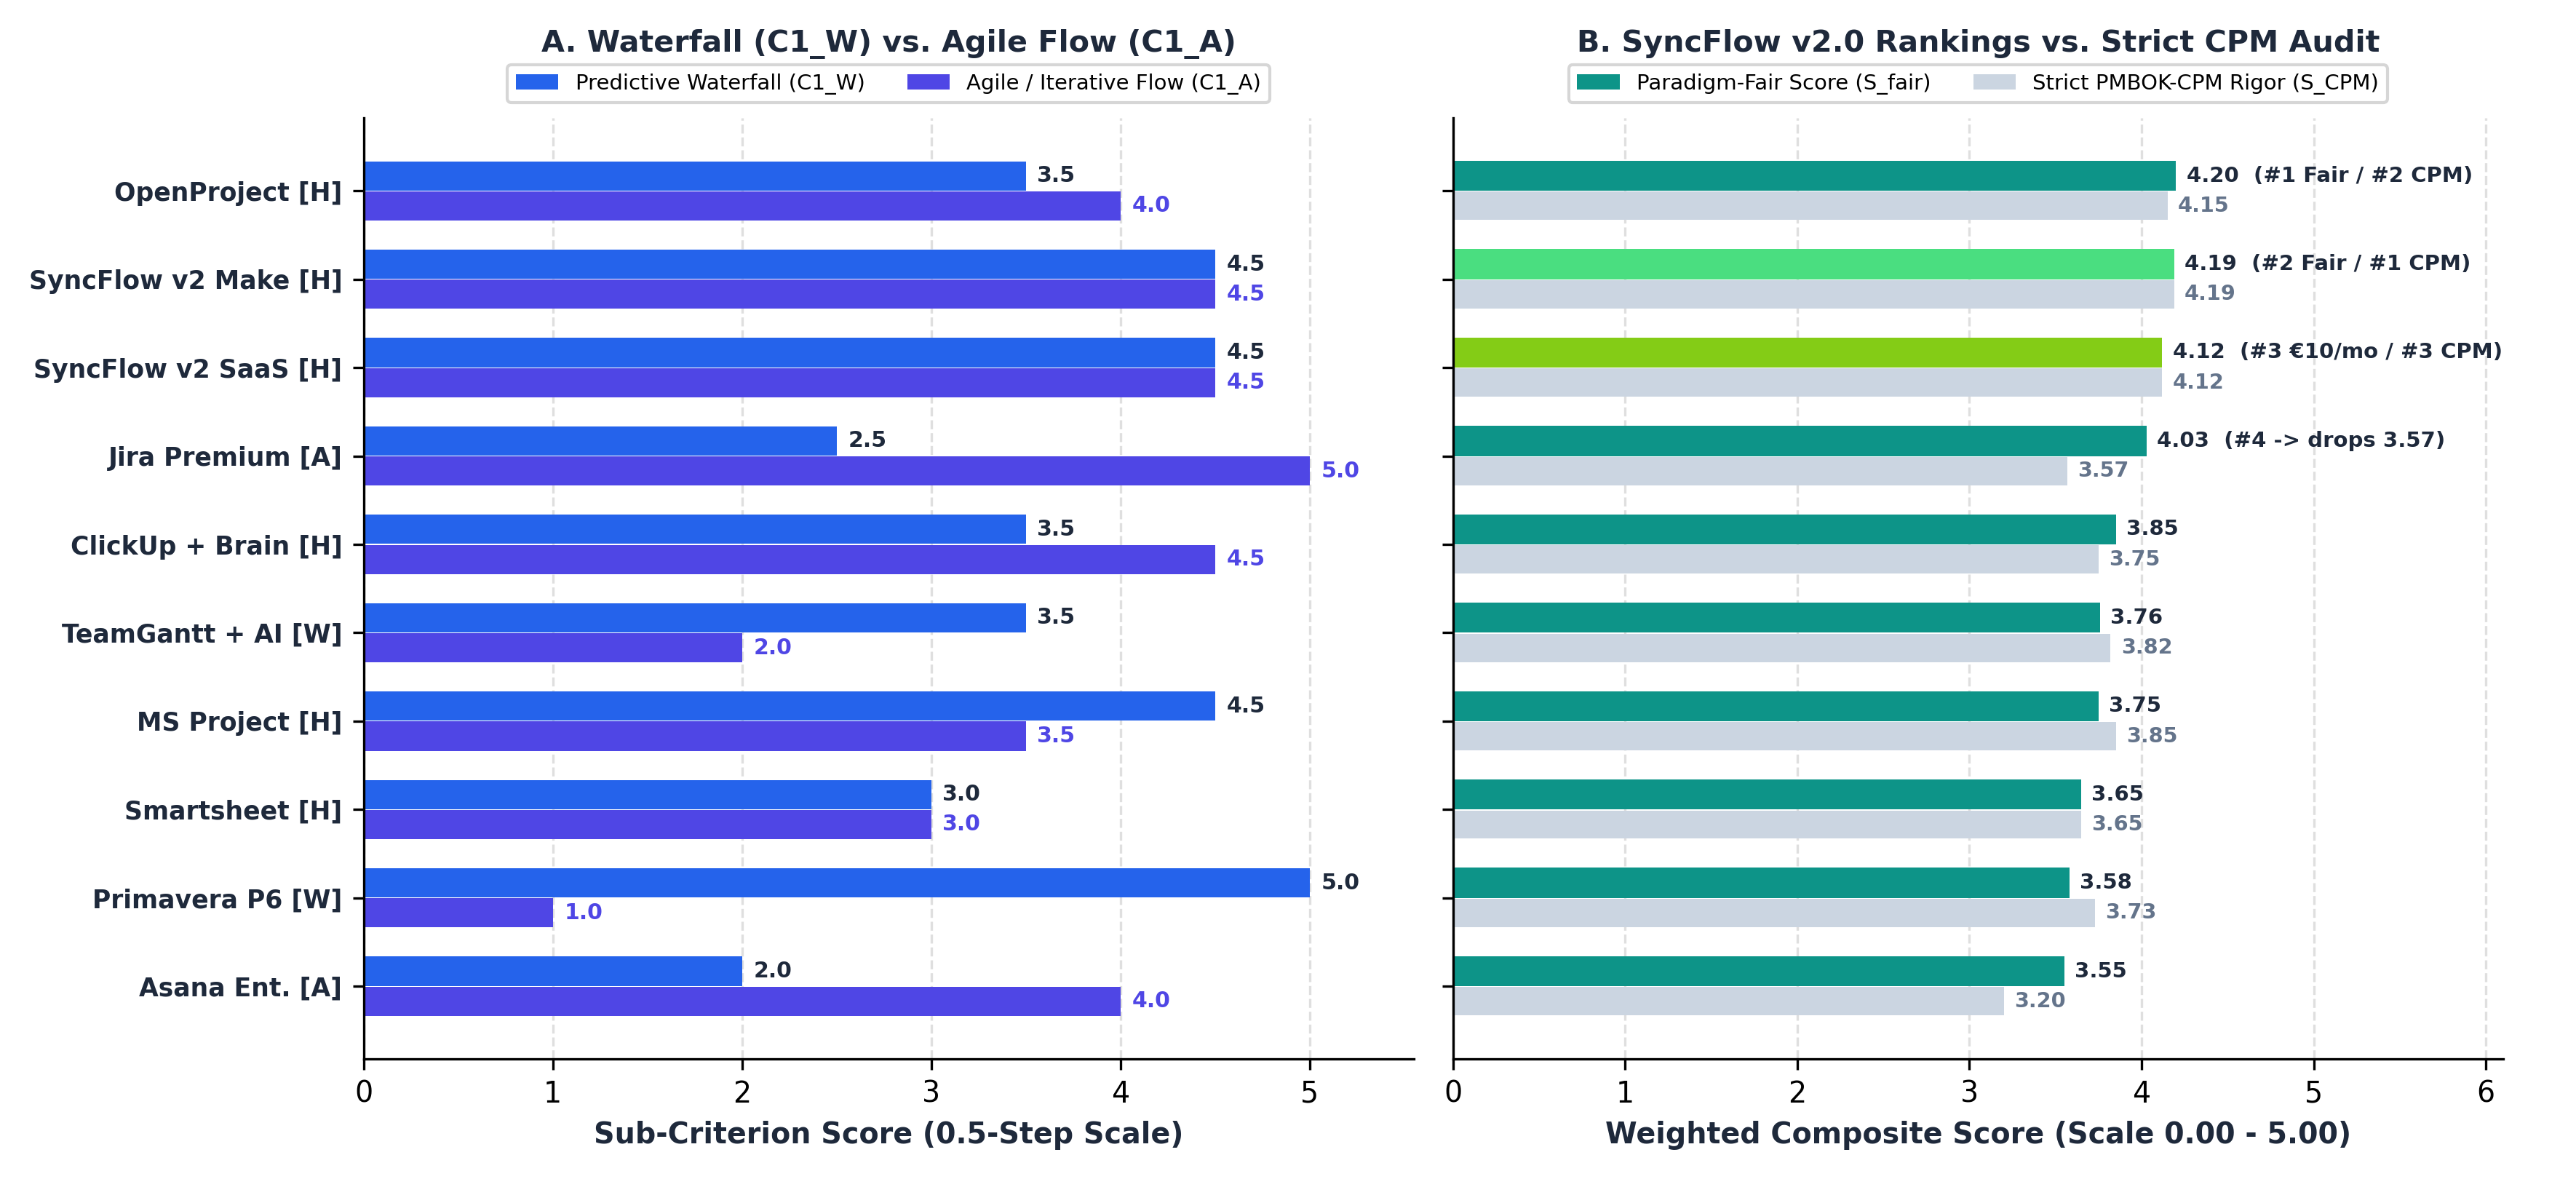
\includegraphics[width=\textwidth]{images/va_v2_weighted_scores.png}
		\caption*{(a) SyncFlow v2.0 comparative profiles.}
	\end{minipage}\hfill
	\begin{minipage}[b]{0.5\textwidth}
		\centering
		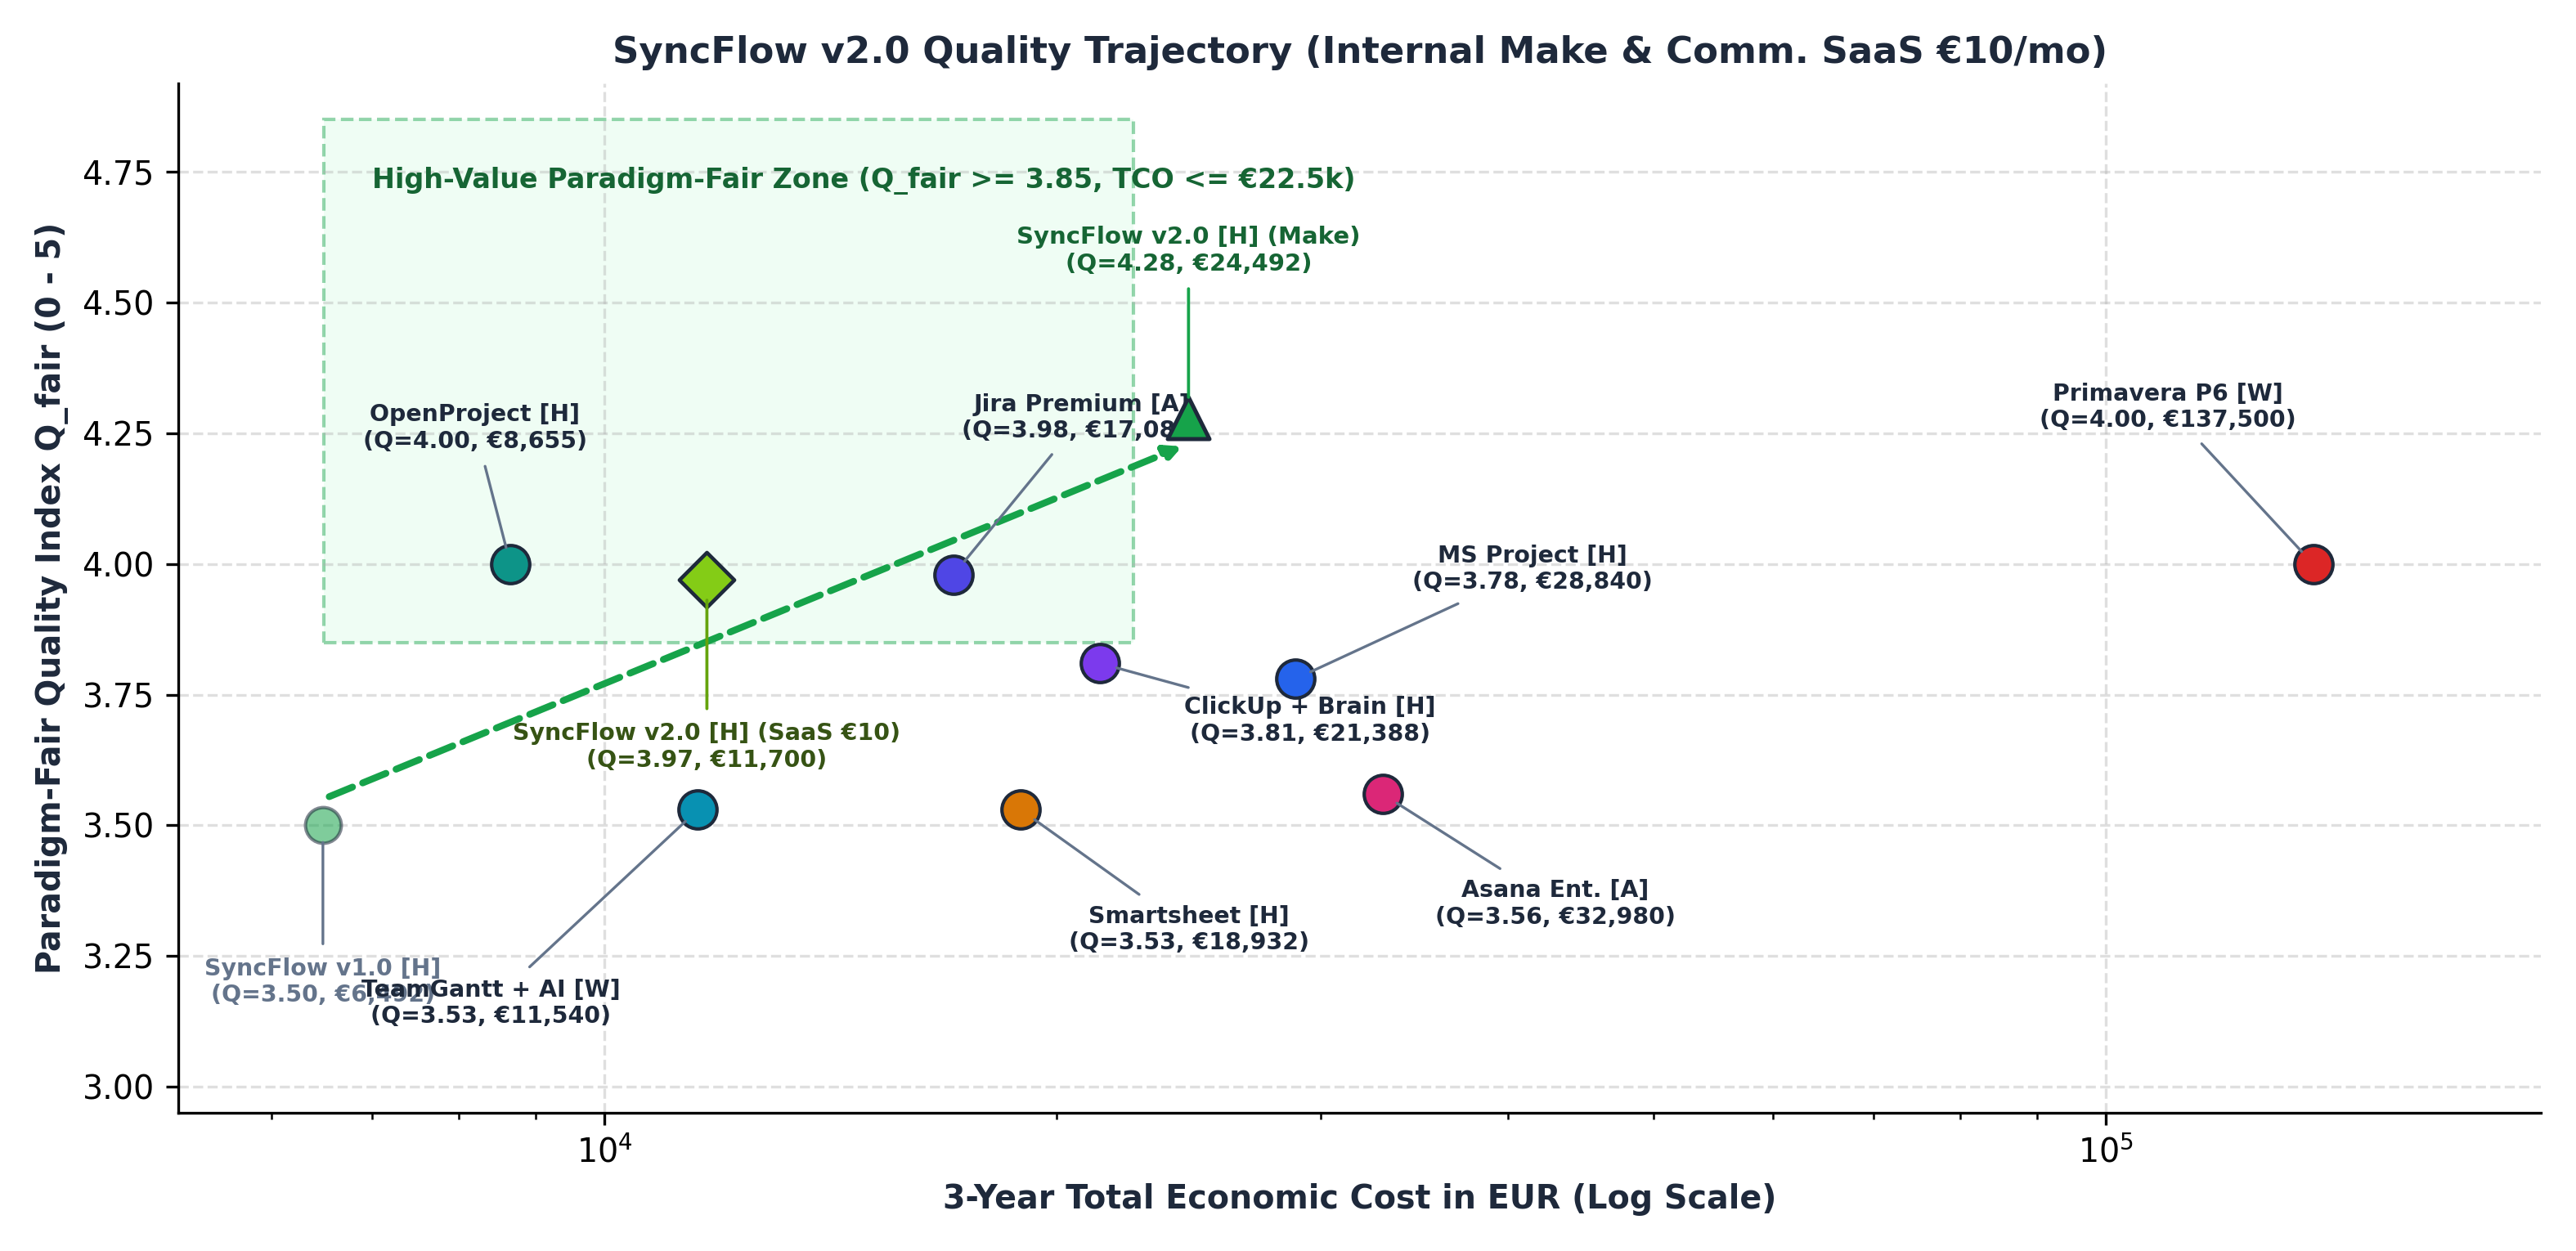
\includegraphics[width=\textwidth]{images/va_v2_value_quadrant.png}
		\caption*{(b) Position in the High-Value quadrant.}
	\end{minipage}
	\vspace{-1mm}
	\caption*{Comparative performance profiles and value efficiency quadrant for the ten evaluated platforms.}
\end{figure}

\noindent \textbf{Time-to-Value and Phased Deployment Strategy.} While commercial SaaS platforms reach operational readiness in 36 hours (€1,620 deployment), building SyncFlow v2.0 requires 400 engineering hours over six months. To ensure immediate scheduling capabilities without delaying organizational adoption, a three-phase deployment is executed:

\begin{itemize}[itemsep=1pt,topsep=1.5pt]
	\item \textbf{Immediate Baseline Production (Day 1)}: Deploy the hardened SyncFlow v1.0 Docker stack. All 25 users immediately access Kahn-based topological sort, CPM forward and backward passes, Gaussian PERT confidence intervals, 14-point DCMA schedule audits, four-stage deliverable quality gates, and duration-based EVM metrics ($PV_t, EV_t, SV_t, SPI_t$).
	\item \textbf{Interim Operational Bridging (Months 1--6)}: During the 6-month v2.0 development sprint on staging branches, missing modules are bridged via standardized PMO procedures:
	\begin{itemize}[itemsep=0.5pt,topsep=0.5pt]
		\item \textit{Monetary Cost EVM}: Team members log active working hours via the v1.0 timer. Project Controllers retrieve verified actual hours through the \path{/completed-activities} REST endpoint and import them into PMO financial templates ($w_h = \text{€45/h}$) to compute financial metrics ($CV, CPI, EAC$).
		\item \textit{Risk Management}: Schedule uncertainties are tracked using a qualitative Risk Register aligned with PMBOK Process 11.2 prior to deploying the automated Monte Carlo engine.
	\end{itemize}
	\item \textbf{Zero-Downtime v2.0 Production Cutover (Month 6)}: At Month 6, staging code is merged. A migration script decouples \texttt{time\_logs} into the new indexed collection, followed by an atomic \texttt{docker compose pull \&\& docker compose up -d} restart. Existing schedule graphs, baselines, and historical time logs are preserved without operational interruption.
\end{itemize}
